\documentclass[twoside]{book}

% Packages required by doxygen
\usepackage{fixltx2e}
\usepackage{calc}
\usepackage{doxygen}
\usepackage{graphicx}
\usepackage[utf8]{inputenc}
\usepackage{makeidx}
\usepackage{multicol}
\usepackage{multirow}
\PassOptionsToPackage{warn}{textcomp}
\usepackage{textcomp}
\usepackage[nointegrals]{wasysym}
\usepackage[table]{xcolor}

% Font selection
\usepackage[T1]{fontenc}
\usepackage{mathptmx}
\usepackage[scaled=.90]{helvet}
\usepackage{courier}
\usepackage{amssymb}
\usepackage{sectsty}
\renewcommand{\familydefault}{\sfdefault}
\allsectionsfont{%
  \fontseries{bc}\selectfont%
  \color{darkgray}%
}
\renewcommand{\DoxyLabelFont}{%
  \fontseries{bc}\selectfont%
  \color{darkgray}%
}
\newcommand{\+}{\discretionary{\mbox{\scriptsize$\hookleftarrow$}}{}{}}

% Page & text layout
\usepackage{geometry}
\geometry{%
  a4paper,%
  top=2.5cm,%
  bottom=2.5cm,%
  left=2.5cm,%
  right=2.5cm%
}
\tolerance=750
\hfuzz=15pt
\hbadness=750
\setlength{\emergencystretch}{15pt}
\setlength{\parindent}{0cm}
\setlength{\parskip}{0.2cm}
\makeatletter
\renewcommand{\paragraph}{%
  \@startsection{paragraph}{4}{0ex}{-1.0ex}{1.0ex}{%
    \normalfont\normalsize\bfseries\SS@parafont%
  }%
}
\renewcommand{\subparagraph}{%
  \@startsection{subparagraph}{5}{0ex}{-1.0ex}{1.0ex}{%
    \normalfont\normalsize\bfseries\SS@subparafont%
  }%
}
\makeatother

% Headers & footers
\usepackage{fancyhdr}
\pagestyle{fancyplain}
\fancyhead[LE]{\fancyplain{}{\bfseries\thepage}}
\fancyhead[CE]{\fancyplain{}{}}
\fancyhead[RE]{\fancyplain{}{\bfseries\leftmark}}
\fancyhead[LO]{\fancyplain{}{\bfseries\rightmark}}
\fancyhead[CO]{\fancyplain{}{}}
\fancyhead[RO]{\fancyplain{}{\bfseries\thepage}}
\fancyfoot[LE]{\fancyplain{}{}}
\fancyfoot[CE]{\fancyplain{}{}}
\fancyfoot[RE]{\fancyplain{}{\bfseries\scriptsize Generated on Sun Mar 27 2016 12\+:01\+:52 for Aqa\+Server by Doxygen }}
\fancyfoot[LO]{\fancyplain{}{\bfseries\scriptsize Generated on Sun Mar 27 2016 12\+:01\+:52 for Aqa\+Server by Doxygen }}
\fancyfoot[CO]{\fancyplain{}{}}
\fancyfoot[RO]{\fancyplain{}{}}
\renewcommand{\footrulewidth}{0.4pt}
\renewcommand{\chaptermark}[1]{%
  \markboth{#1}{}%
}
\renewcommand{\sectionmark}[1]{%
  \markright{\thesection\ #1}%
}

% Indices & bibliography
\usepackage{natbib}
\usepackage[titles]{tocloft}
\setcounter{tocdepth}{3}
\setcounter{secnumdepth}{5}
\makeindex

% Hyperlinks (required, but should be loaded last)
\usepackage{ifpdf}
\ifpdf
  \usepackage[pdftex,pagebackref=true]{hyperref}
\else
  \usepackage[ps2pdf,pagebackref=true]{hyperref}
\fi
\hypersetup{%
  colorlinks=true,%
  linkcolor=blue,%
  citecolor=blue,%
  unicode%
}

% Custom commands
\newcommand{\clearemptydoublepage}{%
  \newpage{\pagestyle{empty}\cleardoublepage}%
}


%===== C O N T E N T S =====

\begin{document}

% Titlepage & ToC
\hypersetup{pageanchor=false,
             bookmarks=true,
             bookmarksnumbered=true,
             pdfencoding=unicode
            }
\pagenumbering{roman}
\begin{titlepage}
\vspace*{7cm}
\begin{center}%
{\Large Aqa\+Server }\\
\vspace*{1cm}
{\large Generated by Doxygen 1.8.7}\\
\vspace*{0.5cm}
{\small Sun Mar 27 2016 12:01:52}\\
\end{center}
\end{titlepage}
\clearemptydoublepage
\tableofcontents
\clearemptydoublepage
\pagenumbering{arabic}
\hypersetup{pageanchor=true}

%--- Begin generated contents ---
\chapter{Main Page}
\label{index}\hypertarget{index}{}Small app for Arduino Uno for aquarium management.

It's suppose to manage\+:
\begin{DoxyItemize}
\item water level,
\item temperature in tank,
\item time to sleep/morning,
\item feeding.
\end{DoxyItemize}

\subsection*{Scheme}

 
\chapter{Class Index}
\section{Class List}
Here are the classes, structs, unions and interfaces with brief descriptions\+:\begin{DoxyCompactList}
\item\contentsline{section}{\hyperlink{struct_tmr}{Tmr} \\*Timer class for containg timers like wake time or sleep time }{\pageref{struct_tmr}}{}
\end{DoxyCompactList}

\chapter{File Index}
\section{File List}
Here is a list of all files with brief descriptions\+:\begin{DoxyCompactList}
\item\contentsline{section}{\hyperlink{_aqa_server_8ino}{Aqa\+Server.\+ino} }{\pageref{_aqa_server_8ino}}{}
\item\contentsline{section}{\hyperlink{feeder_8cpp}{feeder.\+cpp} }{\pageref{feeder_8cpp}}{}
\item\contentsline{section}{\hyperlink{feeder_8h}{feeder.\+h} }{\pageref{feeder_8h}}{}
\item\contentsline{section}{\hyperlink{relay_8cpp}{relay.\+cpp} }{\pageref{relay_8cpp}}{}
\item\contentsline{section}{\hyperlink{relay_8h}{relay.\+h} }{\pageref{relay_8h}}{}
\item\contentsline{section}{\hyperlink{surf_8cpp}{surf.\+cpp} }{\pageref{surf_8cpp}}{}
\item\contentsline{section}{\hyperlink{surf_8h}{surf.\+h} }{\pageref{surf_8h}}{}
\item\contentsline{section}{\hyperlink{temp_8cpp}{temp.\+cpp} }{\pageref{temp_8cpp}}{}
\item\contentsline{section}{\hyperlink{temp_8h}{temp.\+h} }{\pageref{temp_8h}}{}
\item\contentsline{section}{\hyperlink{timent_8cpp}{timent.\+cpp} }{\pageref{timent_8cpp}}{}
\item\contentsline{section}{\hyperlink{timent_8h}{timent.\+h} }{\pageref{timent_8h}}{}
\item\contentsline{section}{\hyperlink{timers_8cpp}{timers.\+cpp} }{\pageref{timers_8cpp}}{}
\item\contentsline{section}{\hyperlink{timers_8h}{timers.\+h} }{\pageref{timers_8h}}{}
\end{DoxyCompactList}

\chapter{Class Documentation}
\hypertarget{struct_tmr}{\section{Tmr Class Reference}
\label{struct_tmr}\index{Tmr@{Tmr}}
}


Timer class for containg timers like wake time or sleep time.  




{\ttfamily \#include $<$timers.\+h$>$}

\subsection*{Public Attributes}
\begin{DoxyCompactItemize}
\item 
byte \hyperlink{struct_tmr_ab0374a7fbe830064a06fb13512453ffa}{h}
\begin{DoxyCompactList}\small\item\em Hour of timer. \end{DoxyCompactList}\item 
byte \hyperlink{struct_tmr_a554c428f359f6d17e82324b0c7568f1a}{m}
\begin{DoxyCompactList}\small\item\em Minute of timer. \end{DoxyCompactList}\item 
byte \hyperlink{struct_tmr_a66e7dcd2c90cb3c25d6410dd1039a2b2}{done}
\begin{DoxyCompactList}\small\item\em Flag if time was set. \end{DoxyCompactList}\end{DoxyCompactItemize}


\subsection{Detailed Description}
Timer class for containg timers like wake time or sleep time. 

Definition at line 9 of file timers.\+h.



\subsection{Member Data Documentation}
\hypertarget{struct_tmr_a66e7dcd2c90cb3c25d6410dd1039a2b2}{\index{Tmr@{Tmr}!done@{done}}
\index{done@{done}!Tmr@{Tmr}}
\subsubsection[{done}]{\setlength{\rightskip}{0pt plus 5cm}byte Tmr\+::done}}\label{struct_tmr_a66e7dcd2c90cb3c25d6410dd1039a2b2}


Flag if time was set. 



Definition at line 12 of file timers.\+h.

\hypertarget{struct_tmr_ab0374a7fbe830064a06fb13512453ffa}{\index{Tmr@{Tmr}!h@{h}}
\index{h@{h}!Tmr@{Tmr}}
\subsubsection[{h}]{\setlength{\rightskip}{0pt plus 5cm}byte Tmr\+::h}}\label{struct_tmr_ab0374a7fbe830064a06fb13512453ffa}


Hour of timer. 



Definition at line 10 of file timers.\+h.

\hypertarget{struct_tmr_a554c428f359f6d17e82324b0c7568f1a}{\index{Tmr@{Tmr}!m@{m}}
\index{m@{m}!Tmr@{Tmr}}
\subsubsection[{m}]{\setlength{\rightskip}{0pt plus 5cm}byte Tmr\+::m}}\label{struct_tmr_a554c428f359f6d17e82324b0c7568f1a}


Minute of timer. 



Definition at line 11 of file timers.\+h.



The documentation for this class was generated from the following file\+:\begin{DoxyCompactItemize}
\item 
\hyperlink{timers_8h}{timers.\+h}\end{DoxyCompactItemize}

\chapter{File Documentation}
\hypertarget{_aqa_server_8ino}{\section{Aqa\+Server.\+ino File Reference}
\label{_aqa_server_8ino}\index{Aqa\+Server.\+ino@{Aqa\+Server.\+ino}}
}
{\ttfamily \#include \char`\"{}relay.\+h\char`\"{}}\\*
{\ttfamily \#include \char`\"{}surf.\+h\char`\"{}}\\*
{\ttfamily \#include \char`\"{}temp.\+h\char`\"{}}\\*
{\ttfamily \#include \char`\"{}timent.\+h\char`\"{}}\\*
{\ttfamily \#include \char`\"{}feeder.\+h\char`\"{}}\\*
{\ttfamily \#include \char`\"{}timers.\+h\char`\"{}}\\*
{\ttfamily \#include $<$E\+E\+P\+R\+O\+M.\+h$>$}\\*
{\ttfamily \#include $<$Ethernet.\+h$>$}\\*
Include dependency graph for Aqa\+Server.\+ino\+:\nopagebreak
\begin{figure}[H]
\begin{center}
\leavevmode
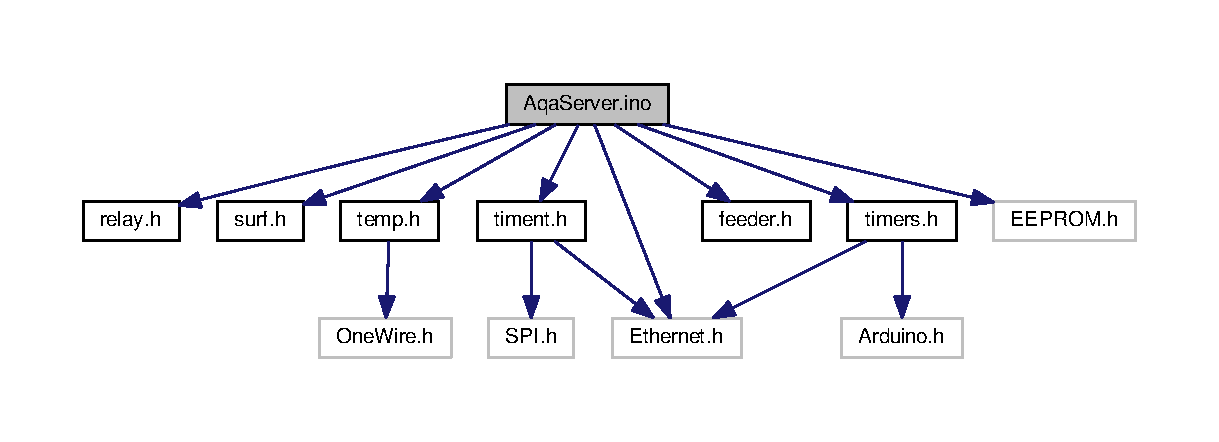
\includegraphics[width=350pt]{_aqa_server_8ino__incl}
\end{center}
\end{figure}
\subsection*{Macros}
\begin{DoxyCompactItemize}
\item 
\#define \hyperlink{_aqa_server_8ino_a1b83ef6dcb797171631472c31018beef}{B\+F\+S}~10
\begin{DoxyCompactList}\small\item\em Size of input buffer. \end{DoxyCompactList}\end{DoxyCompactItemize}
\subsection*{Functions}
\begin{DoxyCompactItemize}
\item 
Ethernet\+Server \hyperlink{_aqa_server_8ino_a0d0f1af61ef5b9c8c9ac1ab61f99dd04}{server} (9011)
\begin{DoxyCompactList}\small\item\em Server instance for port 9011. \end{DoxyCompactList}\item 
void \hyperlink{_aqa_server_8ino_a1d04139db3a5ad5713ecbd14d97da879}{setup} ()
\begin{DoxyCompactList}\small\item\em Setting up all the inputs/outputs. \end{DoxyCompactList}\item 
void \hyperlink{_aqa_server_8ino_a11debc633c690ca19cb27df5f971d73d}{loop} ()
\begin{DoxyCompactList}\small\item\em Looping the Arduino. \end{DoxyCompactList}\end{DoxyCompactItemize}
\subsection*{Variables}
\begin{DoxyCompactItemize}
\item 
byte \hyperlink{_aqa_server_8ino_a50d8813b28b1fc9d3695b4c352fc1f73}{gateway} \mbox{[}$\,$\mbox{]} = \{ 10, 0, 0, 138 \}
\begin{DoxyCompactList}\small\item\em I\+P adress of gateway. \end{DoxyCompactList}\item 
byte \hyperlink{_aqa_server_8ino_a5785acd9d4432010fb73dc54d352ccc3}{subnet} \mbox{[}$\,$\mbox{]} = \{ 255, 255, 255, 0\}
\begin{DoxyCompactList}\small\item\em Network mask adress of Arduino. \end{DoxyCompactList}\end{DoxyCompactItemize}


\subsection{Macro Definition Documentation}
\hypertarget{_aqa_server_8ino_a1b83ef6dcb797171631472c31018beef}{\index{Aqa\+Server.\+ino@{Aqa\+Server.\+ino}!B\+F\+S@{B\+F\+S}}
\index{B\+F\+S@{B\+F\+S}!Aqa\+Server.\+ino@{Aqa\+Server.\+ino}}
\subsubsection[{B\+F\+S}]{\setlength{\rightskip}{0pt plus 5cm}\#define B\+F\+S~10}}\label{_aqa_server_8ino_a1b83ef6dcb797171631472c31018beef}


Size of input buffer. 



Definition at line 31 of file Aqa\+Server.\+ino.



\subsection{Function Documentation}
\hypertarget{_aqa_server_8ino_a11debc633c690ca19cb27df5f971d73d}{\index{Aqa\+Server.\+ino@{Aqa\+Server.\+ino}!loop@{loop}}
\index{loop@{loop}!Aqa\+Server.\+ino@{Aqa\+Server.\+ino}}
\subsubsection[{loop}]{\setlength{\rightskip}{0pt plus 5cm}loop (
\begin{DoxyParamCaption}
{}
\end{DoxyParamCaption}
)}}\label{_aqa_server_8ino_a11debc633c690ca19cb27df5f971d73d}


Looping the Arduino. 



Definition at line 73 of file Aqa\+Server.\+ino.

\hypertarget{_aqa_server_8ino_a0d0f1af61ef5b9c8c9ac1ab61f99dd04}{\index{Aqa\+Server.\+ino@{Aqa\+Server.\+ino}!server@{server}}
\index{server@{server}!Aqa\+Server.\+ino@{Aqa\+Server.\+ino}}
\subsubsection[{server}]{\setlength{\rightskip}{0pt plus 5cm}Ethernet\+Server server (
\begin{DoxyParamCaption}
\item[{9011}]{}
\end{DoxyParamCaption}
)}}\label{_aqa_server_8ino_a0d0f1af61ef5b9c8c9ac1ab61f99dd04}


Server instance for port 9011. 

\hypertarget{_aqa_server_8ino_a1d04139db3a5ad5713ecbd14d97da879}{\index{Aqa\+Server.\+ino@{Aqa\+Server.\+ino}!setup@{setup}}
\index{setup@{setup}!Aqa\+Server.\+ino@{Aqa\+Server.\+ino}}
\subsubsection[{setup}]{\setlength{\rightskip}{0pt plus 5cm}setup (
\begin{DoxyParamCaption}
{}
\end{DoxyParamCaption}
)}}\label{_aqa_server_8ino_a1d04139db3a5ad5713ecbd14d97da879}


Setting up all the inputs/outputs. 



Definition at line 48 of file Aqa\+Server.\+ino.



\subsection{Variable Documentation}
\hypertarget{_aqa_server_8ino_a50d8813b28b1fc9d3695b4c352fc1f73}{\index{Aqa\+Server.\+ino@{Aqa\+Server.\+ino}!gateway@{gateway}}
\index{gateway@{gateway}!Aqa\+Server.\+ino@{Aqa\+Server.\+ino}}
\subsubsection[{gateway}]{\setlength{\rightskip}{0pt plus 5cm}byte gateway\mbox{[}$\,$\mbox{]} = \{ 10, 0, 0, 138 \}}}\label{_aqa_server_8ino_a50d8813b28b1fc9d3695b4c352fc1f73}


I\+P adress of gateway. 



Definition at line 39 of file Aqa\+Server.\+ino.

\hypertarget{_aqa_server_8ino_a5785acd9d4432010fb73dc54d352ccc3}{\index{Aqa\+Server.\+ino@{Aqa\+Server.\+ino}!subnet@{subnet}}
\index{subnet@{subnet}!Aqa\+Server.\+ino@{Aqa\+Server.\+ino}}
\subsubsection[{subnet}]{\setlength{\rightskip}{0pt plus 5cm}byte subnet\mbox{[}$\,$\mbox{]} = \{ 255, 255, 255, 0\}}}\label{_aqa_server_8ino_a5785acd9d4432010fb73dc54d352ccc3}


Network mask adress of Arduino. 



Definition at line 40 of file Aqa\+Server.\+ino.


\hypertarget{feeder_8cpp}{\section{feeder.\+cpp File Reference}
\label{feeder_8cpp}\index{feeder.\+cpp@{feeder.\+cpp}}
}
{\ttfamily \#include \char`\"{}feeder.\+h\char`\"{}}\\*
{\ttfamily \#include $<$Arduino.\+h$>$}\\*
Include dependency graph for feeder.\+cpp\+:
\nopagebreak
\begin{figure}[H]
\begin{center}
\leavevmode
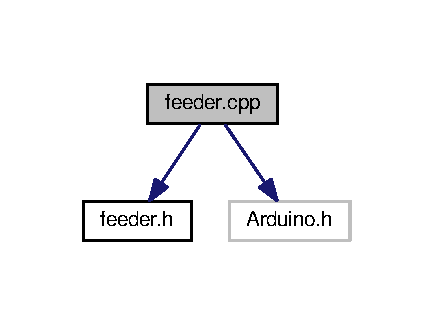
\includegraphics[width=208pt]{feeder_8cpp__incl}
\end{center}
\end{figure}
\subsection*{Functions}
\begin{DoxyCompactItemize}
\item 
void \hyperlink{feeder_8cpp_a0e01e563004702c9043375eb96e4ac16}{init\+Feed} ()
\begin{DoxyCompactList}\small\item\em Step motor initiation. \end{DoxyCompactList}\item 
void \hyperlink{feeder_8cpp_a4d8a16aad63ef59aec6534630b81da88}{turn\+Around} ()
\begin{DoxyCompactList}\small\item\em Turning step motor one time around. \end{DoxyCompactList}\end{DoxyCompactItemize}


\subsection{Function Documentation}
\hypertarget{feeder_8cpp_a0e01e563004702c9043375eb96e4ac16}{\index{feeder.\+cpp@{feeder.\+cpp}!init\+Feed@{init\+Feed}}
\index{init\+Feed@{init\+Feed}!feeder.\+cpp@{feeder.\+cpp}}
\subsubsection[{init\+Feed}]{\setlength{\rightskip}{0pt plus 5cm}init\+Feed (
\begin{DoxyParamCaption}
{}
\end{DoxyParamCaption}
)}}\label{feeder_8cpp_a0e01e563004702c9043375eb96e4ac16}


Step motor initiation. 



Definition at line 8 of file feeder.\+cpp.

\hypertarget{feeder_8cpp_a4d8a16aad63ef59aec6534630b81da88}{\index{feeder.\+cpp@{feeder.\+cpp}!turn\+Around@{turn\+Around}}
\index{turn\+Around@{turn\+Around}!feeder.\+cpp@{feeder.\+cpp}}
\subsubsection[{turn\+Around}]{\setlength{\rightskip}{0pt plus 5cm}turn\+Around (
\begin{DoxyParamCaption}
{}
\end{DoxyParamCaption}
)}}\label{feeder_8cpp_a4d8a16aad63ef59aec6534630b81da88}


Turning step motor one time around. 



Definition at line 16 of file feeder.\+cpp.


\hypertarget{feeder_8h}{\section{feeder.\+h File Reference}
\label{feeder_8h}\index{feeder.\+h@{feeder.\+h}}
}
This graph shows which files directly or indirectly include this file\+:
\nopagebreak
\begin{figure}[H]
\begin{center}
\leavevmode
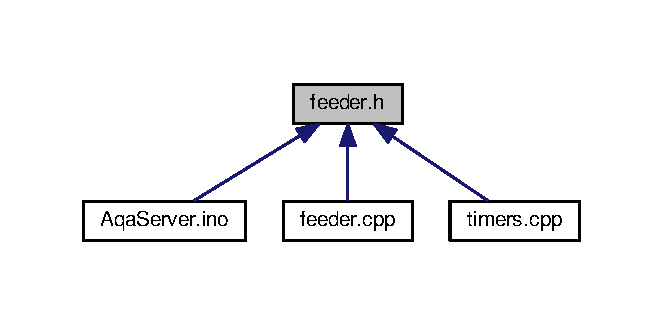
\includegraphics[width=318pt]{feeder_8h__dep__incl}
\end{center}
\end{figure}
\subsection*{Macros}
\begin{DoxyCompactItemize}
\item 
\#define \hyperlink{feeder_8h_a00173d34140b5436cb5b0d11228e1c95}{motor\+Pin1}~6
\begin{DoxyCompactList}\small\item\em Pin number of step motor. \end{DoxyCompactList}\item 
\#define \hyperlink{feeder_8h_ae1842772e10d7a72d3a773ccf17762d0}{motor\+Pin2}~7
\begin{DoxyCompactList}\small\item\em Pin number of step motor. \end{DoxyCompactList}\item 
\#define \hyperlink{feeder_8h_ac3cb6e6fc1af0c626aba727eca3ed466}{motor\+Pin3}~8
\begin{DoxyCompactList}\small\item\em Pin number of step motor. \end{DoxyCompactList}\item 
\#define \hyperlink{feeder_8h_a1d1c0fa5a0378f7c260b60f5d2dab71b}{motor\+Pin4}~9
\begin{DoxyCompactList}\small\item\em Pin number of step motor. \end{DoxyCompactList}\item 
\#define \hyperlink{feeder_8h_a9dcc454a4d70498138f21035a2bf36b9}{delay\+Time}~10
\begin{DoxyCompactList}\small\item\em Time delay at turning. \end{DoxyCompactList}\end{DoxyCompactItemize}
\subsection*{Functions}
\begin{DoxyCompactItemize}
\item 
void \hyperlink{feeder_8h_a5fe976dab21b52a2b537fb88b015c1db}{init\+Feed} ()
\begin{DoxyCompactList}\small\item\em Step motor initiation. \end{DoxyCompactList}\item 
void \hyperlink{feeder_8h_a30ab4062310f87ecf886181e45d520b9}{turn\+Around} ()
\begin{DoxyCompactList}\small\item\em Turning step motor one time around. \end{DoxyCompactList}\end{DoxyCompactItemize}


\subsection{Macro Definition Documentation}
\hypertarget{feeder_8h_a9dcc454a4d70498138f21035a2bf36b9}{\index{feeder.\+h@{feeder.\+h}!delay\+Time@{delay\+Time}}
\index{delay\+Time@{delay\+Time}!feeder.\+h@{feeder.\+h}}
\subsubsection[{delay\+Time}]{\setlength{\rightskip}{0pt plus 5cm}\#define delay\+Time~10}}\label{feeder_8h_a9dcc454a4d70498138f21035a2bf36b9}


Time delay at turning. 



Definition at line 7 of file feeder.\+h.

\hypertarget{feeder_8h_a00173d34140b5436cb5b0d11228e1c95}{\index{feeder.\+h@{feeder.\+h}!motor\+Pin1@{motor\+Pin1}}
\index{motor\+Pin1@{motor\+Pin1}!feeder.\+h@{feeder.\+h}}
\subsubsection[{motor\+Pin1}]{\setlength{\rightskip}{0pt plus 5cm}\#define motor\+Pin1~6}}\label{feeder_8h_a00173d34140b5436cb5b0d11228e1c95}


Pin number of step motor. 



Definition at line 3 of file feeder.\+h.

\hypertarget{feeder_8h_ae1842772e10d7a72d3a773ccf17762d0}{\index{feeder.\+h@{feeder.\+h}!motor\+Pin2@{motor\+Pin2}}
\index{motor\+Pin2@{motor\+Pin2}!feeder.\+h@{feeder.\+h}}
\subsubsection[{motor\+Pin2}]{\setlength{\rightskip}{0pt plus 5cm}\#define motor\+Pin2~7}}\label{feeder_8h_ae1842772e10d7a72d3a773ccf17762d0}


Pin number of step motor. 



Definition at line 4 of file feeder.\+h.

\hypertarget{feeder_8h_ac3cb6e6fc1af0c626aba727eca3ed466}{\index{feeder.\+h@{feeder.\+h}!motor\+Pin3@{motor\+Pin3}}
\index{motor\+Pin3@{motor\+Pin3}!feeder.\+h@{feeder.\+h}}
\subsubsection[{motor\+Pin3}]{\setlength{\rightskip}{0pt plus 5cm}\#define motor\+Pin3~8}}\label{feeder_8h_ac3cb6e6fc1af0c626aba727eca3ed466}


Pin number of step motor. 



Definition at line 5 of file feeder.\+h.

\hypertarget{feeder_8h_a1d1c0fa5a0378f7c260b60f5d2dab71b}{\index{feeder.\+h@{feeder.\+h}!motor\+Pin4@{motor\+Pin4}}
\index{motor\+Pin4@{motor\+Pin4}!feeder.\+h@{feeder.\+h}}
\subsubsection[{motor\+Pin4}]{\setlength{\rightskip}{0pt plus 5cm}\#define motor\+Pin4~9}}\label{feeder_8h_a1d1c0fa5a0378f7c260b60f5d2dab71b}


Pin number of step motor. 



Definition at line 6 of file feeder.\+h.



\subsection{Function Documentation}
\hypertarget{feeder_8h_a5fe976dab21b52a2b537fb88b015c1db}{\index{feeder.\+h@{feeder.\+h}!init\+Feed@{init\+Feed}}
\index{init\+Feed@{init\+Feed}!feeder.\+h@{feeder.\+h}}
\subsubsection[{init\+Feed}]{\setlength{\rightskip}{0pt plus 5cm}void init\+Feed (
\begin{DoxyParamCaption}
{}
\end{DoxyParamCaption}
)}}\label{feeder_8h_a5fe976dab21b52a2b537fb88b015c1db}


Step motor initiation. 



Definition at line 8 of file feeder.\+cpp.

\hypertarget{feeder_8h_a30ab4062310f87ecf886181e45d520b9}{\index{feeder.\+h@{feeder.\+h}!turn\+Around@{turn\+Around}}
\index{turn\+Around@{turn\+Around}!feeder.\+h@{feeder.\+h}}
\subsubsection[{turn\+Around}]{\setlength{\rightskip}{0pt plus 5cm}void turn\+Around (
\begin{DoxyParamCaption}
{}
\end{DoxyParamCaption}
)}}\label{feeder_8h_a30ab4062310f87ecf886181e45d520b9}


Turning step motor one time around. 



Definition at line 16 of file feeder.\+cpp.


\hypertarget{_r_e_a_d_m_e_8md}{\section{R\+E\+A\+D\+M\+E.\+md File Reference}
\label{_r_e_a_d_m_e_8md}\index{R\+E\+A\+D\+M\+E.\+md@{R\+E\+A\+D\+M\+E.\+md}}
}

\hypertarget{relay_8cpp}{\section{relay.\+cpp File Reference}
\label{relay_8cpp}\index{relay.\+cpp@{relay.\+cpp}}
}
{\ttfamily \#include \char`\"{}relay.\+h\char`\"{}}\\*
{\ttfamily \#include $<$Arduino.\+h$>$}\\*
Include dependency graph for relay.\+cpp\+:
\nopagebreak
\begin{figure}[H]
\begin{center}
\leavevmode
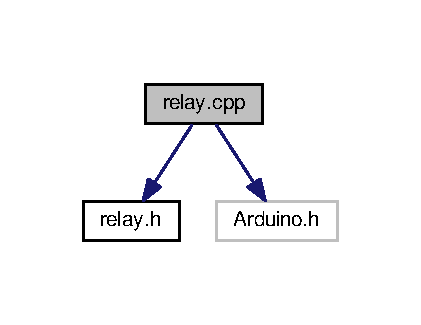
\includegraphics[width=202pt]{relay_8cpp__incl}
\end{center}
\end{figure}
\subsection*{Functions}
\begin{DoxyCompactItemize}
\item 
void \hyperlink{relay_8cpp_a77d2d1fc9580fc4e47c0b47bc8f78752}{init\+Relays} ()
\begin{DoxyCompactList}\small\item\em Relay initiation. \end{DoxyCompactList}\item 
void \hyperlink{relay_8cpp_a02140e5c577d206c5ee42415032e3b57}{switch\+Relay} (int x)
\begin{DoxyCompactList}\small\item\em Switch relay given by x to different state. \end{DoxyCompactList}\item 
void \hyperlink{relay_8cpp_a7764566d1e0c4cd31cf200e00d2f4843}{switch\+Set} (int x, int state)
\begin{DoxyCompactList}\small\item\em Set the realy state by given x. \end{DoxyCompactList}\item 
void \hyperlink{relay_8cpp_aa237259c6c5f5cc60a2dbcdb62961346}{switch\+On} (int x)
\begin{DoxyCompactList}\small\item\em Switch off relay state by the given x. \end{DoxyCompactList}\item 
void \hyperlink{relay_8cpp_a2ee42df8fba1ea7c0a86e77f94ad6680}{switch\+Off} (int x)
\begin{DoxyCompactList}\small\item\em Switch off relay state by the given x. \end{DoxyCompactList}\item 
int \hyperlink{relay_8cpp_aebbe632e173506016c4586de2af372e0}{switch\+State} (int x)
\begin{DoxyCompactList}\small\item\em Getter for relay state by the given x. \end{DoxyCompactList}\end{DoxyCompactItemize}
\subsection*{Variables}
\begin{DoxyCompactItemize}
\item 
int \hyperlink{relay_8cpp_a31f225c55d9a4421ae5cf5a48bc084b6}{relays\+\_\+stats} \mbox{[}\hyperlink{relay_8h_a1a6cf8977361352646bc8ec84b4466b7}{R\+E\+L\+A\+Y\+\_\+\+C\+N\+T}\mbox{]}
\begin{DoxyCompactList}\small\item\em Relay status array. \end{DoxyCompactList}\end{DoxyCompactItemize}


\subsection{Function Documentation}
\hypertarget{relay_8cpp_a77d2d1fc9580fc4e47c0b47bc8f78752}{\index{relay.\+cpp@{relay.\+cpp}!init\+Relays@{init\+Relays}}
\index{init\+Relays@{init\+Relays}!relay.\+cpp@{relay.\+cpp}}
\subsubsection[{init\+Relays}]{\setlength{\rightskip}{0pt plus 5cm}init\+Relays (
\begin{DoxyParamCaption}
{}
\end{DoxyParamCaption}
)}}\label{relay_8cpp_a77d2d1fc9580fc4e47c0b47bc8f78752}


Relay initiation. 



Definition at line 9 of file relay.\+cpp.

\hypertarget{relay_8cpp_a2ee42df8fba1ea7c0a86e77f94ad6680}{\index{relay.\+cpp@{relay.\+cpp}!switch\+Off@{switch\+Off}}
\index{switch\+Off@{switch\+Off}!relay.\+cpp@{relay.\+cpp}}
\subsubsection[{switch\+Off}]{\setlength{\rightskip}{0pt plus 5cm}switch\+Off (
\begin{DoxyParamCaption}
\item[{int}]{x}
\end{DoxyParamCaption}
)}}\label{relay_8cpp_a2ee42df8fba1ea7c0a86e77f94ad6680}


Switch off relay state by the given x. 


\begin{DoxyParams}{Parameters}
{\em x} & Number of relay. \\
\hline
\end{DoxyParams}


Definition at line 32 of file relay.\+cpp.

\hypertarget{relay_8cpp_aa237259c6c5f5cc60a2dbcdb62961346}{\index{relay.\+cpp@{relay.\+cpp}!switch\+On@{switch\+On}}
\index{switch\+On@{switch\+On}!relay.\+cpp@{relay.\+cpp}}
\subsubsection[{switch\+On}]{\setlength{\rightskip}{0pt plus 5cm}switch\+On (
\begin{DoxyParamCaption}
\item[{int}]{x}
\end{DoxyParamCaption}
)}}\label{relay_8cpp_aa237259c6c5f5cc60a2dbcdb62961346}


Switch off relay state by the given x. 


\begin{DoxyParams}{Parameters}
{\em x} & Number of relay. \\
\hline
\end{DoxyParams}


Definition at line 26 of file relay.\+cpp.

\hypertarget{relay_8cpp_a02140e5c577d206c5ee42415032e3b57}{\index{relay.\+cpp@{relay.\+cpp}!switch\+Relay@{switch\+Relay}}
\index{switch\+Relay@{switch\+Relay}!relay.\+cpp@{relay.\+cpp}}
\subsubsection[{switch\+Relay}]{\setlength{\rightskip}{0pt plus 5cm}switch\+Relay (
\begin{DoxyParamCaption}
\item[{int}]{x}
\end{DoxyParamCaption}
)}}\label{relay_8cpp_a02140e5c577d206c5ee42415032e3b57}


Switch relay given by x to different state. 


\begin{DoxyParams}{Parameters}
{\em x} & Number of relay \\
\hline
\end{DoxyParams}


Definition at line 18 of file relay.\+cpp.

\hypertarget{relay_8cpp_a7764566d1e0c4cd31cf200e00d2f4843}{\index{relay.\+cpp@{relay.\+cpp}!switch\+Set@{switch\+Set}}
\index{switch\+Set@{switch\+Set}!relay.\+cpp@{relay.\+cpp}}
\subsubsection[{switch\+Set}]{\setlength{\rightskip}{0pt plus 5cm}switch\+Set (
\begin{DoxyParamCaption}
\item[{int}]{x, }
\item[{int}]{state}
\end{DoxyParamCaption}
)}}\label{relay_8cpp_a7764566d1e0c4cd31cf200e00d2f4843}


Set the realy state by given x. 


\begin{DoxyParams}{Parameters}
{\em x} & Number of relay. \\
\hline
{\em state} & New state of relay. \\
\hline
\end{DoxyParams}


Definition at line 22 of file relay.\+cpp.

\hypertarget{relay_8cpp_aebbe632e173506016c4586de2af372e0}{\index{relay.\+cpp@{relay.\+cpp}!switch\+State@{switch\+State}}
\index{switch\+State@{switch\+State}!relay.\+cpp@{relay.\+cpp}}
\subsubsection[{switch\+State}]{\setlength{\rightskip}{0pt plus 5cm}switch\+State (
\begin{DoxyParamCaption}
\item[{int}]{x}
\end{DoxyParamCaption}
)}}\label{relay_8cpp_aebbe632e173506016c4586de2af372e0}


Getter for relay state by the given x. 


\begin{DoxyParams}{Parameters}
{\em x} & Number of relay. \\
\hline
\end{DoxyParams}
\begin{DoxyReturn}{Returns}
State of relay. 
\end{DoxyReturn}


Definition at line 38 of file relay.\+cpp.



\subsection{Variable Documentation}
\hypertarget{relay_8cpp_a31f225c55d9a4421ae5cf5a48bc084b6}{\index{relay.\+cpp@{relay.\+cpp}!relays\+\_\+stats@{relays\+\_\+stats}}
\index{relays\+\_\+stats@{relays\+\_\+stats}!relay.\+cpp@{relay.\+cpp}}
\subsubsection[{relays\+\_\+stats}]{\setlength{\rightskip}{0pt plus 5cm}int relays\+\_\+stats\mbox{[}{\bf R\+E\+L\+A\+Y\+\_\+\+C\+N\+T}\mbox{]}}}\label{relay_8cpp_a31f225c55d9a4421ae5cf5a48bc084b6}


Relay status array. 



Definition at line 4 of file relay.\+cpp.


\hypertarget{relay_8h}{\section{relay.\+h File Reference}
\label{relay_8h}\index{relay.\+h@{relay.\+h}}
}
This graph shows which files directly or indirectly include this file\+:
\nopagebreak
\begin{figure}[H]
\begin{center}
\leavevmode
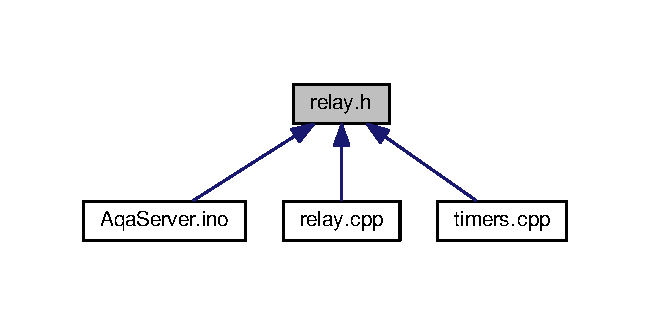
\includegraphics[width=312pt]{relay_8h__dep__incl}
\end{center}
\end{figure}
\subsection*{Macros}
\begin{DoxyCompactItemize}
\item 
\#define \hyperlink{relay_8h_a1a6cf8977361352646bc8ec84b4466b7}{R\+E\+L\+A\+Y\+\_\+\+C\+N\+T}~3
\begin{DoxyCompactList}\small\item\em Number of relays. \end{DoxyCompactList}\item 
\#define \hyperlink{relay_8h_a3d6b4709b64f79ea4b9d2cc8df9e4aed}{L\+I\+G\+H\+T\+S}~3
\begin{DoxyCompactList}\small\item\em Light pin relay. \end{DoxyCompactList}\item 
\#define \hyperlink{relay_8h_a3a9cb517ac5b9aeae4caa398a0ed07cd}{F\+I\+L\+T\+E\+R}~4
\begin{DoxyCompactList}\small\item\em Filter pin relay. \end{DoxyCompactList}\item 
\#define \hyperlink{relay_8h_a242cc70f67d2a4caee37bea7bb5e4007}{H\+E\+A\+T\+E\+R}~5
\begin{DoxyCompactList}\small\item\em Heater pin relay. \end{DoxyCompactList}\end{DoxyCompactItemize}
\subsection*{Functions}
\begin{DoxyCompactItemize}
\item 
void \hyperlink{relay_8h_a1978a69e69c52fe9cb779046030bf001}{init\+Relays} ()
\begin{DoxyCompactList}\small\item\em Relay initiation. \end{DoxyCompactList}\item 
void \hyperlink{relay_8h_a93797aafa292711b664f829f89d71756}{switch\+Relay} (int x)
\begin{DoxyCompactList}\small\item\em Switch relay given by x to different state. \end{DoxyCompactList}\item 
void \hyperlink{relay_8h_afb7ec8c8b937d057cd4eefb361d3d844}{switch\+Set} (int x, int state)
\begin{DoxyCompactList}\small\item\em Set the realy state by given x. \end{DoxyCompactList}\item 
void \hyperlink{relay_8h_a538380d744a4e47fc5d61f0f64c137b9}{switch\+On} (int x)
\begin{DoxyCompactList}\small\item\em Switch off relay state by the given x. \end{DoxyCompactList}\item 
void \hyperlink{relay_8h_a998dea521719e4774f007bef1744c9f4}{switch\+Off} (int x)
\begin{DoxyCompactList}\small\item\em Switch off relay state by the given x. \end{DoxyCompactList}\item 
int \hyperlink{relay_8h_a0b2793ce4156256c0037b45be06d6cd0}{switch\+State} (int x)
\begin{DoxyCompactList}\small\item\em Getter for relay state by the given x. \end{DoxyCompactList}\end{DoxyCompactItemize}


\subsection{Macro Definition Documentation}
\hypertarget{relay_8h_a3a9cb517ac5b9aeae4caa398a0ed07cd}{\index{relay.\+h@{relay.\+h}!F\+I\+L\+T\+E\+R@{F\+I\+L\+T\+E\+R}}
\index{F\+I\+L\+T\+E\+R@{F\+I\+L\+T\+E\+R}!relay.\+h@{relay.\+h}}
\subsubsection[{F\+I\+L\+T\+E\+R}]{\setlength{\rightskip}{0pt plus 5cm}\#define F\+I\+L\+T\+E\+R~4}}\label{relay_8h_a3a9cb517ac5b9aeae4caa398a0ed07cd}


Filter pin relay. 



Definition at line 5 of file relay.\+h.

\hypertarget{relay_8h_a242cc70f67d2a4caee37bea7bb5e4007}{\index{relay.\+h@{relay.\+h}!H\+E\+A\+T\+E\+R@{H\+E\+A\+T\+E\+R}}
\index{H\+E\+A\+T\+E\+R@{H\+E\+A\+T\+E\+R}!relay.\+h@{relay.\+h}}
\subsubsection[{H\+E\+A\+T\+E\+R}]{\setlength{\rightskip}{0pt plus 5cm}\#define H\+E\+A\+T\+E\+R~5}}\label{relay_8h_a242cc70f67d2a4caee37bea7bb5e4007}


Heater pin relay. 



Definition at line 6 of file relay.\+h.

\hypertarget{relay_8h_a3d6b4709b64f79ea4b9d2cc8df9e4aed}{\index{relay.\+h@{relay.\+h}!L\+I\+G\+H\+T\+S@{L\+I\+G\+H\+T\+S}}
\index{L\+I\+G\+H\+T\+S@{L\+I\+G\+H\+T\+S}!relay.\+h@{relay.\+h}}
\subsubsection[{L\+I\+G\+H\+T\+S}]{\setlength{\rightskip}{0pt plus 5cm}\#define L\+I\+G\+H\+T\+S~3}}\label{relay_8h_a3d6b4709b64f79ea4b9d2cc8df9e4aed}


Light pin relay. 



Definition at line 4 of file relay.\+h.

\hypertarget{relay_8h_a1a6cf8977361352646bc8ec84b4466b7}{\index{relay.\+h@{relay.\+h}!R\+E\+L\+A\+Y\+\_\+\+C\+N\+T@{R\+E\+L\+A\+Y\+\_\+\+C\+N\+T}}
\index{R\+E\+L\+A\+Y\+\_\+\+C\+N\+T@{R\+E\+L\+A\+Y\+\_\+\+C\+N\+T}!relay.\+h@{relay.\+h}}
\subsubsection[{R\+E\+L\+A\+Y\+\_\+\+C\+N\+T}]{\setlength{\rightskip}{0pt plus 5cm}\#define R\+E\+L\+A\+Y\+\_\+\+C\+N\+T~3}}\label{relay_8h_a1a6cf8977361352646bc8ec84b4466b7}


Number of relays. 



Definition at line 3 of file relay.\+h.



\subsection{Function Documentation}
\hypertarget{relay_8h_a1978a69e69c52fe9cb779046030bf001}{\index{relay.\+h@{relay.\+h}!init\+Relays@{init\+Relays}}
\index{init\+Relays@{init\+Relays}!relay.\+h@{relay.\+h}}
\subsubsection[{init\+Relays}]{\setlength{\rightskip}{0pt plus 5cm}void init\+Relays (
\begin{DoxyParamCaption}
{}
\end{DoxyParamCaption}
)}}\label{relay_8h_a1978a69e69c52fe9cb779046030bf001}


Relay initiation. 



Definition at line 9 of file relay.\+cpp.

\hypertarget{relay_8h_a998dea521719e4774f007bef1744c9f4}{\index{relay.\+h@{relay.\+h}!switch\+Off@{switch\+Off}}
\index{switch\+Off@{switch\+Off}!relay.\+h@{relay.\+h}}
\subsubsection[{switch\+Off}]{\setlength{\rightskip}{0pt plus 5cm}void switch\+Off (
\begin{DoxyParamCaption}
\item[{int}]{x}
\end{DoxyParamCaption}
)}}\label{relay_8h_a998dea521719e4774f007bef1744c9f4}


Switch off relay state by the given x. 


\begin{DoxyParams}{Parameters}
{\em x} & Number of relay. \\
\hline
\end{DoxyParams}


Definition at line 32 of file relay.\+cpp.

\hypertarget{relay_8h_a538380d744a4e47fc5d61f0f64c137b9}{\index{relay.\+h@{relay.\+h}!switch\+On@{switch\+On}}
\index{switch\+On@{switch\+On}!relay.\+h@{relay.\+h}}
\subsubsection[{switch\+On}]{\setlength{\rightskip}{0pt plus 5cm}void switch\+On (
\begin{DoxyParamCaption}
\item[{int}]{x}
\end{DoxyParamCaption}
)}}\label{relay_8h_a538380d744a4e47fc5d61f0f64c137b9}


Switch off relay state by the given x. 


\begin{DoxyParams}{Parameters}
{\em x} & Number of relay. \\
\hline
\end{DoxyParams}


Definition at line 26 of file relay.\+cpp.

\hypertarget{relay_8h_a93797aafa292711b664f829f89d71756}{\index{relay.\+h@{relay.\+h}!switch\+Relay@{switch\+Relay}}
\index{switch\+Relay@{switch\+Relay}!relay.\+h@{relay.\+h}}
\subsubsection[{switch\+Relay}]{\setlength{\rightskip}{0pt plus 5cm}void switch\+Relay (
\begin{DoxyParamCaption}
\item[{int}]{x}
\end{DoxyParamCaption}
)}}\label{relay_8h_a93797aafa292711b664f829f89d71756}


Switch relay given by x to different state. 


\begin{DoxyParams}{Parameters}
{\em x} & Number of relay \\
\hline
\end{DoxyParams}


Definition at line 18 of file relay.\+cpp.

\hypertarget{relay_8h_afb7ec8c8b937d057cd4eefb361d3d844}{\index{relay.\+h@{relay.\+h}!switch\+Set@{switch\+Set}}
\index{switch\+Set@{switch\+Set}!relay.\+h@{relay.\+h}}
\subsubsection[{switch\+Set}]{\setlength{\rightskip}{0pt plus 5cm}void switch\+Set (
\begin{DoxyParamCaption}
\item[{int}]{x, }
\item[{int}]{state}
\end{DoxyParamCaption}
)}}\label{relay_8h_afb7ec8c8b937d057cd4eefb361d3d844}


Set the realy state by given x. 


\begin{DoxyParams}{Parameters}
{\em x} & Number of relay. \\
\hline
{\em state} & New state of relay. \\
\hline
\end{DoxyParams}


Definition at line 22 of file relay.\+cpp.

\hypertarget{relay_8h_a0b2793ce4156256c0037b45be06d6cd0}{\index{relay.\+h@{relay.\+h}!switch\+State@{switch\+State}}
\index{switch\+State@{switch\+State}!relay.\+h@{relay.\+h}}
\subsubsection[{switch\+State}]{\setlength{\rightskip}{0pt plus 5cm}int switch\+State (
\begin{DoxyParamCaption}
\item[{int}]{x}
\end{DoxyParamCaption}
)}}\label{relay_8h_a0b2793ce4156256c0037b45be06d6cd0}


Getter for relay state by the given x. 


\begin{DoxyParams}{Parameters}
{\em x} & Number of relay. \\
\hline
\end{DoxyParams}
\begin{DoxyReturn}{Returns}
State of relay. 
\end{DoxyReturn}


Definition at line 38 of file relay.\+cpp.


\hypertarget{surf_8cpp}{\section{surf.\+cpp File Reference}
\label{surf_8cpp}\index{surf.\+cpp@{surf.\+cpp}}
}
{\ttfamily \#include \char`\"{}surf.\+h\char`\"{}}\\*
{\ttfamily \#include $<$Arduino.\+h$>$}\\*
Include dependency graph for surf.\+cpp\+:\nopagebreak
\begin{figure}[H]
\begin{center}
\leavevmode
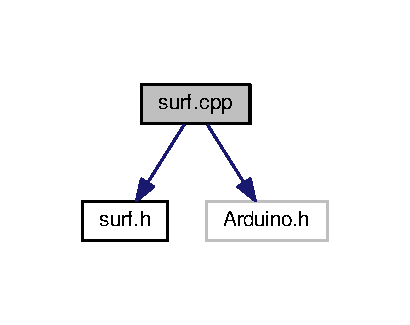
\includegraphics[width=197pt]{surf_8cpp__incl}
\end{center}
\end{figure}
\subsection*{Functions}
\begin{DoxyCompactItemize}
\item 
void \hyperlink{surf_8cpp_aeb728321a15d1de94a55a61f935a745b}{init\+Surface} ()
\begin{DoxyCompactList}\small\item\em Relay initiation. \end{DoxyCompactList}\item 
int \hyperlink{surf_8cpp_a282b0af88968ac8e268c0f21cdf5f034}{get\+Surface} ()
\begin{DoxyCompactList}\small\item\em Relay status getter. \end{DoxyCompactList}\end{DoxyCompactItemize}


\subsection{Function Documentation}
\hypertarget{surf_8cpp_a282b0af88968ac8e268c0f21cdf5f034}{\index{surf.\+cpp@{surf.\+cpp}!get\+Surface@{get\+Surface}}
\index{get\+Surface@{get\+Surface}!surf.\+cpp@{surf.\+cpp}}
\subsubsection[{get\+Surface}]{\setlength{\rightskip}{0pt plus 5cm}get\+Surface (
\begin{DoxyParamCaption}
{}
\end{DoxyParamCaption}
)}}\label{surf_8cpp_a282b0af88968ac8e268c0f21cdf5f034}


Relay status getter. 

\begin{DoxyReturn}{Returns}
The state of switch. 
\end{DoxyReturn}


Definition at line 11 of file surf.\+cpp.

\hypertarget{surf_8cpp_aeb728321a15d1de94a55a61f935a745b}{\index{surf.\+cpp@{surf.\+cpp}!init\+Surface@{init\+Surface}}
\index{init\+Surface@{init\+Surface}!surf.\+cpp@{surf.\+cpp}}
\subsubsection[{init\+Surface}]{\setlength{\rightskip}{0pt plus 5cm}init\+Surface (
\begin{DoxyParamCaption}
{}
\end{DoxyParamCaption}
)}}\label{surf_8cpp_aeb728321a15d1de94a55a61f935a745b}


Relay initiation. 



Definition at line 7 of file surf.\+cpp.


\hypertarget{surf_8h}{\section{surf.\+h File Reference}
\label{surf_8h}\index{surf.\+h@{surf.\+h}}
}
This graph shows which files directly or indirectly include this file\+:\nopagebreak
\begin{figure}[H]
\begin{center}
\leavevmode
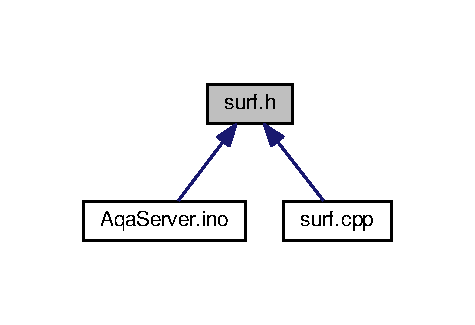
\includegraphics[width=228pt]{surf_8h__dep__incl}
\end{center}
\end{figure}
\subsection*{Macros}
\begin{DoxyCompactItemize}
\item 
\#define \hyperlink{surf_8h_a359da429f8866dc81fd62d64d65e5134}{S\+W\+I\+T\+C\+H\+\_\+\+S\+U\+R}~A0
\begin{DoxyCompactList}\small\item\em Surface switch input pin. \end{DoxyCompactList}\end{DoxyCompactItemize}
\subsection*{Functions}
\begin{DoxyCompactItemize}
\item 
void \hyperlink{surf_8h_ab4520083b29de1f13864036fe1226dfb}{init\+Surface} ()
\begin{DoxyCompactList}\small\item\em Relay initiation. \end{DoxyCompactList}\item 
int \hyperlink{surf_8h_ae2df54c8af473b8a811873ecac1377bc}{get\+Surface} ()
\begin{DoxyCompactList}\small\item\em Relay status getter. \end{DoxyCompactList}\end{DoxyCompactItemize}


\subsection{Macro Definition Documentation}
\hypertarget{surf_8h_a359da429f8866dc81fd62d64d65e5134}{\index{surf.\+h@{surf.\+h}!S\+W\+I\+T\+C\+H\+\_\+\+S\+U\+R@{S\+W\+I\+T\+C\+H\+\_\+\+S\+U\+R}}
\index{S\+W\+I\+T\+C\+H\+\_\+\+S\+U\+R@{S\+W\+I\+T\+C\+H\+\_\+\+S\+U\+R}!surf.\+h@{surf.\+h}}
\subsubsection[{S\+W\+I\+T\+C\+H\+\_\+\+S\+U\+R}]{\setlength{\rightskip}{0pt plus 5cm}\#define S\+W\+I\+T\+C\+H\+\_\+\+S\+U\+R~A0}}\label{surf_8h_a359da429f8866dc81fd62d64d65e5134}


Surface switch input pin. 



Definition at line 3 of file surf.\+h.



\subsection{Function Documentation}
\hypertarget{surf_8h_ae2df54c8af473b8a811873ecac1377bc}{\index{surf.\+h@{surf.\+h}!get\+Surface@{get\+Surface}}
\index{get\+Surface@{get\+Surface}!surf.\+h@{surf.\+h}}
\subsubsection[{get\+Surface}]{\setlength{\rightskip}{0pt plus 5cm}int get\+Surface (
\begin{DoxyParamCaption}
{}
\end{DoxyParamCaption}
)}}\label{surf_8h_ae2df54c8af473b8a811873ecac1377bc}


Relay status getter. 

\begin{DoxyReturn}{Returns}
The state of switch. 
\end{DoxyReturn}


Definition at line 11 of file surf.\+cpp.

\hypertarget{surf_8h_ab4520083b29de1f13864036fe1226dfb}{\index{surf.\+h@{surf.\+h}!init\+Surface@{init\+Surface}}
\index{init\+Surface@{init\+Surface}!surf.\+h@{surf.\+h}}
\subsubsection[{init\+Surface}]{\setlength{\rightskip}{0pt plus 5cm}void init\+Surface (
\begin{DoxyParamCaption}
{}
\end{DoxyParamCaption}
)}}\label{surf_8h_ab4520083b29de1f13864036fe1226dfb}


Relay initiation. 



Definition at line 7 of file surf.\+cpp.


\hypertarget{temp_8cpp}{\section{temp.\+cpp File Reference}
\label{temp_8cpp}\index{temp.\+cpp@{temp.\+cpp}}
}
{\ttfamily \#include \char`\"{}temp.\+h\char`\"{}}\\*
{\ttfamily \#include $<$One\+Wire.\+h$>$}\\*
{\ttfamily \#include $<$Arduino.\+h$>$}\\*
Include dependency graph for temp.\+cpp\+:\nopagebreak
\begin{figure}[H]
\begin{center}
\leavevmode
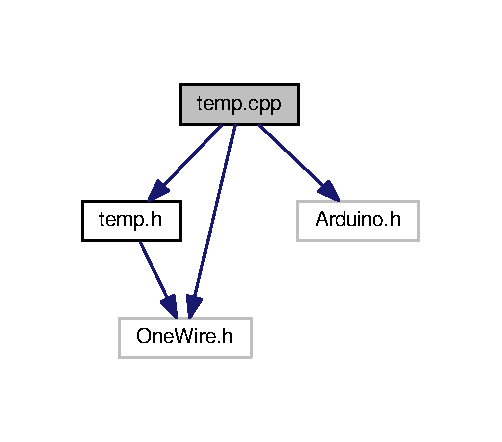
\includegraphics[width=241pt]{temp_8cpp__incl}
\end{center}
\end{figure}
\subsection*{Functions}
\begin{DoxyCompactItemize}
\item 
One\+Wire \hyperlink{temp_8cpp_a56ca5239b99f7efc5530d479b28eb3b5}{ds} (\hyperlink{temp_8cpp_a339051b7625b4a7104be5810c5004a5e}{D\+S18\+S20\+\_\+\+Pin})
\item 
float \hyperlink{temp_8cpp_a404413cc6b56eaa7d34382e2af8668f7}{get\+Temp} ()
\begin{DoxyCompactList}\small\item\em Temperature getter. \end{DoxyCompactList}\end{DoxyCompactItemize}
\subsection*{Variables}
\begin{DoxyCompactItemize}
\item 
int \hyperlink{temp_8cpp_a339051b7625b4a7104be5810c5004a5e}{D\+S18\+S20\+\_\+\+Pin} = 2
\begin{DoxyCompactList}\small\item\em Pin of R\+T\+C. \end{DoxyCompactList}\end{DoxyCompactItemize}


\subsection{Function Documentation}
\hypertarget{temp_8cpp_a56ca5239b99f7efc5530d479b28eb3b5}{\index{temp.\+cpp@{temp.\+cpp}!ds@{ds}}
\index{ds@{ds}!temp.\+cpp@{temp.\+cpp}}
\subsubsection[{ds}]{\setlength{\rightskip}{0pt plus 5cm}One\+Wire ds (
\begin{DoxyParamCaption}
\item[{{\bf D\+S18\+S20\+\_\+\+Pin}}]{}
\end{DoxyParamCaption}
)}}\label{temp_8cpp_a56ca5239b99f7efc5530d479b28eb3b5}
\hypertarget{temp_8cpp_a404413cc6b56eaa7d34382e2af8668f7}{\index{temp.\+cpp@{temp.\+cpp}!get\+Temp@{get\+Temp}}
\index{get\+Temp@{get\+Temp}!temp.\+cpp@{temp.\+cpp}}
\subsubsection[{get\+Temp}]{\setlength{\rightskip}{0pt plus 5cm}get\+Temp (
\begin{DoxyParamCaption}
{}
\end{DoxyParamCaption}
)}}\label{temp_8cpp_a404413cc6b56eaa7d34382e2af8668f7}


Temperature getter. 

\begin{DoxyReturn}{Returns}
Temperature of aqarium. 
\end{DoxyReturn}


Definition at line 11 of file temp.\+cpp.



\subsection{Variable Documentation}
\hypertarget{temp_8cpp_a339051b7625b4a7104be5810c5004a5e}{\index{temp.\+cpp@{temp.\+cpp}!D\+S18\+S20\+\_\+\+Pin@{D\+S18\+S20\+\_\+\+Pin}}
\index{D\+S18\+S20\+\_\+\+Pin@{D\+S18\+S20\+\_\+\+Pin}!temp.\+cpp@{temp.\+cpp}}
\subsubsection[{D\+S18\+S20\+\_\+\+Pin}]{\setlength{\rightskip}{0pt plus 5cm}int D\+S18\+S20\+\_\+\+Pin = 2}}\label{temp_8cpp_a339051b7625b4a7104be5810c5004a5e}


Pin of R\+T\+C. 



Definition at line 5 of file temp.\+cpp.


\hypertarget{temp_8h}{\section{temp.\+h File Reference}
\label{temp_8h}\index{temp.\+h@{temp.\+h}}
}
{\ttfamily \#include $<$One\+Wire.\+h$>$}\\*
Include dependency graph for temp.\+h\+:
\nopagebreak
\begin{figure}[H]
\begin{center}
\leavevmode
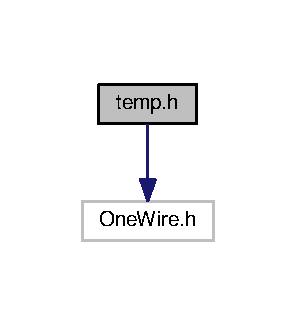
\includegraphics[width=142pt]{temp_8h__incl}
\end{center}
\end{figure}
This graph shows which files directly or indirectly include this file\+:
\nopagebreak
\begin{figure}[H]
\begin{center}
\leavevmode
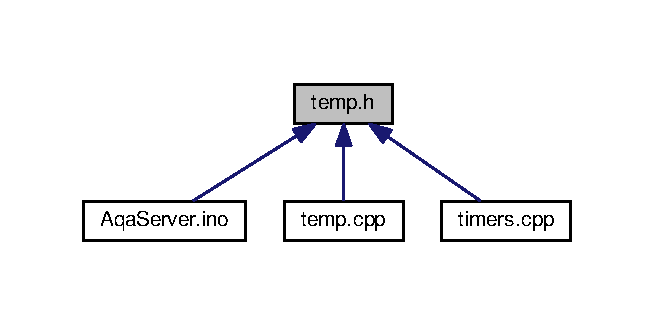
\includegraphics[width=314pt]{temp_8h__dep__incl}
\end{center}
\end{figure}
\subsection*{Functions}
\begin{DoxyCompactItemize}
\item 
float \hyperlink{temp_8h_a6459ed0635e25efb428ae3dfe1cab682}{get\+Temp} ()
\begin{DoxyCompactList}\small\item\em Temperature getter. \end{DoxyCompactList}\end{DoxyCompactItemize}


\subsection{Function Documentation}
\hypertarget{temp_8h_a6459ed0635e25efb428ae3dfe1cab682}{\index{temp.\+h@{temp.\+h}!get\+Temp@{get\+Temp}}
\index{get\+Temp@{get\+Temp}!temp.\+h@{temp.\+h}}
\subsubsection[{get\+Temp}]{\setlength{\rightskip}{0pt plus 5cm}float get\+Temp (
\begin{DoxyParamCaption}
{}
\end{DoxyParamCaption}
)}}\label{temp_8h_a6459ed0635e25efb428ae3dfe1cab682}


Temperature getter. 

\begin{DoxyReturn}{Returns}
Temperature of aqarium. 
\end{DoxyReturn}


Definition at line 11 of file temp.\+cpp.


\hypertarget{timent_8cpp}{\section{timent.\+cpp File Reference}
\label{timent_8cpp}\index{timent.\+cpp@{timent.\+cpp}}
}
{\ttfamily \#include \char`\"{}timent.\+h\char`\"{}}\\*
{\ttfamily \#include $<$S\+P\+I.\+h$>$}\\*
{\ttfamily \#include $<$Ethernet.\+h$>$}\\*
{\ttfamily \#include $<$R\+T\+Clib.\+h$>$}\\*
{\ttfamily \#include \char`\"{}Wire.\+h\char`\"{}}\\*
{\ttfamily \#include $<$Udp.\+h$>$}\\*
Include dependency graph for timent.\+cpp\+:\nopagebreak
\begin{figure}[H]
\begin{center}
\leavevmode
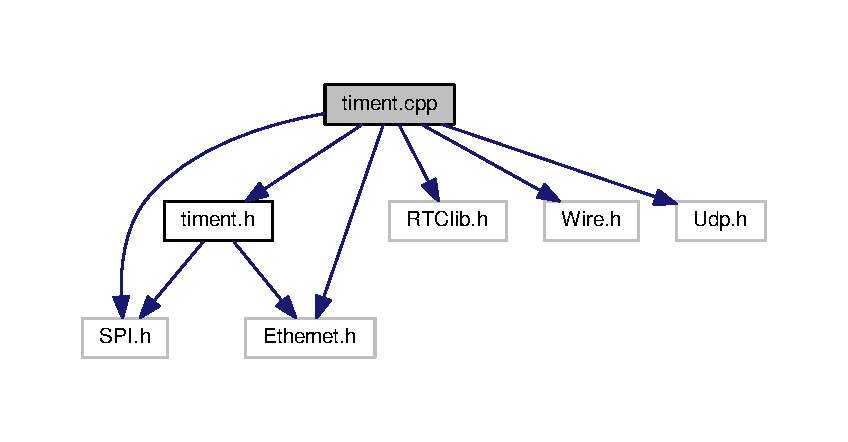
\includegraphics[width=350pt]{timent_8cpp__incl}
\end{center}
\end{figure}
\subsection*{Macros}
\begin{DoxyCompactItemize}
\item 
\#define \hyperlink{timent_8cpp_a5d3e17478bd7215166c197b07edf4efd}{D\+S3231\+\_\+\+I2\+C\+\_\+\+A\+D\+D\+R\+E\+S\+S}~0x68
\end{DoxyCompactItemize}
\subsection*{Functions}
\begin{DoxyCompactItemize}
\item 
void \hyperlink{timent_8cpp_a72baaca6b79ef889dec6298fd01830ab}{init\+Timent} ()
\begin{DoxyCompactList}\small\item\em Init of R\+T\+C. \end{DoxyCompactList}\item 
byte \hyperlink{timent_8cpp_a48adf7e672d1841aa28e85622a25aa80}{dec\+To\+Bcd} (byte val)
\begin{DoxyCompactList}\small\item\em Decadic format to binary coded decimal. \end{DoxyCompactList}\item 
byte \hyperlink{timent_8cpp_ad8941f1405da415e231f96719121d961}{bcd\+To\+Dec} (byte val)
\begin{DoxyCompactList}\small\item\em Binary coded decimal to decadic format. \end{DoxyCompactList}\item 
void \hyperlink{timent_8cpp_acc59d6059cf7d8872c99547e70bb9e00}{set\+D\+S3231time} (byte second, byte \hyperlink{timers_8cpp_a0f100646613882af0415f3d97bd67875}{minute}, byte \hyperlink{timers_8cpp_aafa4b28cd4cce6ab8fbe430b55b647ad}{hour}, byte day\+Of\+Week, byte day\+Of\+Month, byte month, byte year)
\begin{DoxyCompactList}\small\item\em Setter for R\+T\+C. \end{DoxyCompactList}\item 
void \hyperlink{timent_8cpp_a2dc0bfb9c1fa2b144186ae2933d589ea}{read\+D\+S3231\+Minutes\+Houres} (byte $\ast$\hyperlink{timers_8cpp_a0f100646613882af0415f3d97bd67875}{minute}, byte $\ast$\hyperlink{timers_8cpp_aafa4b28cd4cce6ab8fbe430b55b647ad}{hour})
\item 
void \hyperlink{timent_8cpp_a2fb4d2d1f9d3145dcbe0c66f7152b48b}{read\+D\+S3231time} (byte $\ast$second, byte $\ast$\hyperlink{timers_8cpp_a0f100646613882af0415f3d97bd67875}{minute}, byte $\ast$\hyperlink{timers_8cpp_aafa4b28cd4cce6ab8fbe430b55b647ad}{hour}, byte $\ast$day\+Of\+Week, byte $\ast$day\+Of\+Month, byte $\ast$month, byte $\ast$year)
\item 
void \hyperlink{timent_8cpp_adb5769a64028d495d2f1a57e40e99302}{display\+Http\+Time} (Ethernet\+Client $\ast$client)
\begin{DoxyCompactList}\small\item\em Response for ethernet connection for time values. \end{DoxyCompactList}\item 
void \hyperlink{timent_8cpp_a4f1bcabc6a32ffba4de3656ac50e859a}{display\+Time} ()
\begin{DoxyCompactList}\small\item\em Displays time on the console. \end{DoxyCompactList}\item 
unsigned long \hyperlink{timent_8cpp_a1f893cc95960e3189f2c72e2aa58b73c}{send\+N\+T\+Ppacket} (byte $\ast$address)
\begin{DoxyCompactList}\small\item\em Sender of N\+T\+P request to N\+T\+P server given by address. \end{DoxyCompactList}\item 
boolean \hyperlink{timent_8cpp_a591c8fbcb88bbea3648c5bbf1a0fc49e}{set\+Time} ()
\begin{DoxyCompactList}\small\item\em Set time by N\+T\+P server to R\+T\+C. \end{DoxyCompactList}\end{DoxyCompactItemize}
\subsection*{Variables}
\begin{DoxyCompactItemize}
\item 
byte \hyperlink{timent_8cpp_a25ccc714e88d75e5f03801b892611213}{time\+Server} \mbox{[}$\,$\mbox{]} = \{10, 0, 0, 4\}
\begin{DoxyCompactList}\small\item\em Remote N\+T\+P server. \end{DoxyCompactList}\item 
unsigned int \hyperlink{timent_8cpp_ac240824c9b35035b41bc24ee200565a2}{local\+Port} = 31011
\begin{DoxyCompactList}\small\item\em Local T\+C\+P connection port. \end{DoxyCompactList}\item 
const int \hyperlink{timent_8cpp_ae2843b6487d71a38433763495c106346}{N\+T\+P\+\_\+\+P\+A\+C\+K\+E\+T\+\_\+\+S\+I\+Z\+E} = 48
\item 
byte \hyperlink{timent_8cpp_a4cd2b78b3cddeed9e1c5520520da1a81}{pb} \mbox{[}\hyperlink{timent_8cpp_ae2843b6487d71a38433763495c106346}{N\+T\+P\+\_\+\+P\+A\+C\+K\+E\+T\+\_\+\+S\+I\+Z\+E}\mbox{]}
\item 
Ethernet\+U\+D\+P \hyperlink{timent_8cpp_ac12f4a699dd1eac03facdc1ebf3028d4}{Udp}
\end{DoxyCompactItemize}


\subsection{Macro Definition Documentation}
\hypertarget{timent_8cpp_a5d3e17478bd7215166c197b07edf4efd}{\index{timent.\+cpp@{timent.\+cpp}!D\+S3231\+\_\+\+I2\+C\+\_\+\+A\+D\+D\+R\+E\+S\+S@{D\+S3231\+\_\+\+I2\+C\+\_\+\+A\+D\+D\+R\+E\+S\+S}}
\index{D\+S3231\+\_\+\+I2\+C\+\_\+\+A\+D\+D\+R\+E\+S\+S@{D\+S3231\+\_\+\+I2\+C\+\_\+\+A\+D\+D\+R\+E\+S\+S}!timent.\+cpp@{timent.\+cpp}}
\subsubsection[{D\+S3231\+\_\+\+I2\+C\+\_\+\+A\+D\+D\+R\+E\+S\+S}]{\setlength{\rightskip}{0pt plus 5cm}\#define D\+S3231\+\_\+\+I2\+C\+\_\+\+A\+D\+D\+R\+E\+S\+S~0x68}}\label{timent_8cpp_a5d3e17478bd7215166c197b07edf4efd}


Definition at line 6 of file timent.\+cpp.



\subsection{Function Documentation}
\hypertarget{timent_8cpp_ad8941f1405da415e231f96719121d961}{\index{timent.\+cpp@{timent.\+cpp}!bcd\+To\+Dec@{bcd\+To\+Dec}}
\index{bcd\+To\+Dec@{bcd\+To\+Dec}!timent.\+cpp@{timent.\+cpp}}
\subsubsection[{bcd\+To\+Dec}]{\setlength{\rightskip}{0pt plus 5cm}bcd\+To\+Dec (
\begin{DoxyParamCaption}
\item[{byte}]{val}
\end{DoxyParamCaption}
)}}\label{timent_8cpp_ad8941f1405da415e231f96719121d961}


Binary coded decimal to decadic format. 


\begin{DoxyParams}{Parameters}
{\em val} & Binary coded number. \\
\hline
\end{DoxyParams}
\begin{DoxyReturn}{Returns}
Decimal value. 
\end{DoxyReturn}


Definition at line 32 of file timent.\+cpp.

\hypertarget{timent_8cpp_a48adf7e672d1841aa28e85622a25aa80}{\index{timent.\+cpp@{timent.\+cpp}!dec\+To\+Bcd@{dec\+To\+Bcd}}
\index{dec\+To\+Bcd@{dec\+To\+Bcd}!timent.\+cpp@{timent.\+cpp}}
\subsubsection[{dec\+To\+Bcd}]{\setlength{\rightskip}{0pt plus 5cm}dec\+To\+Bcd (
\begin{DoxyParamCaption}
\item[{byte}]{val}
\end{DoxyParamCaption}
)}}\label{timent_8cpp_a48adf7e672d1841aa28e85622a25aa80}


Decadic format to binary coded decimal. 


\begin{DoxyParams}{Parameters}
{\em val} & Decadic number \\
\hline
\end{DoxyParams}
\begin{DoxyReturn}{Returns}
Binary coded decimal value. 
\end{DoxyReturn}


Definition at line 27 of file timent.\+cpp.

\hypertarget{timent_8cpp_adb5769a64028d495d2f1a57e40e99302}{\index{timent.\+cpp@{timent.\+cpp}!display\+Http\+Time@{display\+Http\+Time}}
\index{display\+Http\+Time@{display\+Http\+Time}!timent.\+cpp@{timent.\+cpp}}
\subsubsection[{display\+Http\+Time}]{\setlength{\rightskip}{0pt plus 5cm}display\+Http\+Time (
\begin{DoxyParamCaption}
\item[{Ethernet\+Client $\ast$}]{client}
\end{DoxyParamCaption}
)}}\label{timent_8cpp_adb5769a64028d495d2f1a57e40e99302}


Response for ethernet connection for time values. 


\begin{DoxyParams}{Parameters}
{\em client} & Ethernet client to send the message to. \\
\hline
\end{DoxyParams}


Definition at line 75 of file timent.\+cpp.

\hypertarget{timent_8cpp_a4f1bcabc6a32ffba4de3656ac50e859a}{\index{timent.\+cpp@{timent.\+cpp}!display\+Time@{display\+Time}}
\index{display\+Time@{display\+Time}!timent.\+cpp@{timent.\+cpp}}
\subsubsection[{display\+Time}]{\setlength{\rightskip}{0pt plus 5cm}display\+Time (
\begin{DoxyParamCaption}
{}
\end{DoxyParamCaption}
)}}\label{timent_8cpp_a4f1bcabc6a32ffba4de3656ac50e859a}


Displays time on the console. 



Definition at line 124 of file timent.\+cpp.

\hypertarget{timent_8cpp_a72baaca6b79ef889dec6298fd01830ab}{\index{timent.\+cpp@{timent.\+cpp}!init\+Timent@{init\+Timent}}
\index{init\+Timent@{init\+Timent}!timent.\+cpp@{timent.\+cpp}}
\subsubsection[{init\+Timent}]{\setlength{\rightskip}{0pt plus 5cm}init\+Timent (
\begin{DoxyParamCaption}
{}
\end{DoxyParamCaption}
)}}\label{timent_8cpp_a72baaca6b79ef889dec6298fd01830ab}


Init of R\+T\+C. 



Definition at line 23 of file timent.\+cpp.

\hypertarget{timent_8cpp_a2dc0bfb9c1fa2b144186ae2933d589ea}{\index{timent.\+cpp@{timent.\+cpp}!read\+D\+S3231\+Minutes\+Houres@{read\+D\+S3231\+Minutes\+Houres}}
\index{read\+D\+S3231\+Minutes\+Houres@{read\+D\+S3231\+Minutes\+Houres}!timent.\+cpp@{timent.\+cpp}}
\subsubsection[{read\+D\+S3231\+Minutes\+Houres}]{\setlength{\rightskip}{0pt plus 5cm}void read\+D\+S3231\+Minutes\+Houres (
\begin{DoxyParamCaption}
\item[{byte $\ast$}]{minute, }
\item[{byte $\ast$}]{hour}
\end{DoxyParamCaption}
)}}\label{timent_8cpp_a2dc0bfb9c1fa2b144186ae2933d589ea}


Definition at line 49 of file timent.\+cpp.

\hypertarget{timent_8cpp_a2fb4d2d1f9d3145dcbe0c66f7152b48b}{\index{timent.\+cpp@{timent.\+cpp}!read\+D\+S3231time@{read\+D\+S3231time}}
\index{read\+D\+S3231time@{read\+D\+S3231time}!timent.\+cpp@{timent.\+cpp}}
\subsubsection[{read\+D\+S3231time}]{\setlength{\rightskip}{0pt plus 5cm}void read\+D\+S3231time (
\begin{DoxyParamCaption}
\item[{byte $\ast$}]{second, }
\item[{byte $\ast$}]{minute, }
\item[{byte $\ast$}]{hour, }
\item[{byte $\ast$}]{day\+Of\+Week, }
\item[{byte $\ast$}]{day\+Of\+Month, }
\item[{byte $\ast$}]{month, }
\item[{byte $\ast$}]{year}
\end{DoxyParamCaption}
)}}\label{timent_8cpp_a2fb4d2d1f9d3145dcbe0c66f7152b48b}


Definition at line 60 of file timent.\+cpp.

\hypertarget{timent_8cpp_a1f893cc95960e3189f2c72e2aa58b73c}{\index{timent.\+cpp@{timent.\+cpp}!send\+N\+T\+Ppacket@{send\+N\+T\+Ppacket}}
\index{send\+N\+T\+Ppacket@{send\+N\+T\+Ppacket}!timent.\+cpp@{timent.\+cpp}}
\subsubsection[{send\+N\+T\+Ppacket}]{\setlength{\rightskip}{0pt plus 5cm}send\+N\+T\+Ppacket (
\begin{DoxyParamCaption}
\item[{byte $\ast$}]{address}
\end{DoxyParamCaption}
)}}\label{timent_8cpp_a1f893cc95960e3189f2c72e2aa58b73c}


Sender of N\+T\+P request to N\+T\+P server given by address. 


\begin{DoxyParams}{Parameters}
{\em address} & Address of N\+T\+P server. \\
\hline
\end{DoxyParams}
\begin{DoxyReturn}{Returns}
N\+T\+P time stamp. 
\end{DoxyReturn}


Definition at line 174 of file timent.\+cpp.

\hypertarget{timent_8cpp_acc59d6059cf7d8872c99547e70bb9e00}{\index{timent.\+cpp@{timent.\+cpp}!set\+D\+S3231time@{set\+D\+S3231time}}
\index{set\+D\+S3231time@{set\+D\+S3231time}!timent.\+cpp@{timent.\+cpp}}
\subsubsection[{set\+D\+S3231time}]{\setlength{\rightskip}{0pt plus 5cm}set\+D\+S3231time (
\begin{DoxyParamCaption}
\item[{byte}]{second, }
\item[{byte}]{minute, }
\item[{byte}]{hour, }
\item[{byte}]{day\+Of\+Week, }
\item[{byte}]{day\+Of\+Month, }
\item[{byte}]{month, }
\item[{byte}]{year}
\end{DoxyParamCaption}
)}}\label{timent_8cpp_acc59d6059cf7d8872c99547e70bb9e00}


Setter for R\+T\+C. 


\begin{DoxyParams}{Parameters}
{\em second} & Second of time. \\
\hline
{\em minute} & Minute of time. \\
\hline
{\em hour} & Hours of time \\
\hline
{\em day\+Of\+Week} & Day of the week. \\
\hline
{\em day\+Of\+Month} & Day of the month. \\
\hline
{\em month} & Current month. \\
\hline
{\em year} & Current year. \\
\hline
\end{DoxyParams}


Definition at line 35 of file timent.\+cpp.

\hypertarget{timent_8cpp_a591c8fbcb88bbea3648c5bbf1a0fc49e}{\index{timent.\+cpp@{timent.\+cpp}!set\+Time@{set\+Time}}
\index{set\+Time@{set\+Time}!timent.\+cpp@{timent.\+cpp}}
\subsubsection[{set\+Time}]{\setlength{\rightskip}{0pt plus 5cm}set\+Time (
\begin{DoxyParamCaption}
{}
\end{DoxyParamCaption}
)}}\label{timent_8cpp_a591c8fbcb88bbea3648c5bbf1a0fc49e}


Set time by N\+T\+P server to R\+T\+C. 

\begin{DoxyReturn}{Returns}
Status of time setting. 
\end{DoxyReturn}


Definition at line 194 of file timent.\+cpp.



\subsection{Variable Documentation}
\hypertarget{timent_8cpp_ac240824c9b35035b41bc24ee200565a2}{\index{timent.\+cpp@{timent.\+cpp}!local\+Port@{local\+Port}}
\index{local\+Port@{local\+Port}!timent.\+cpp@{timent.\+cpp}}
\subsubsection[{local\+Port}]{\setlength{\rightskip}{0pt plus 5cm}unsigned int local\+Port = 31011}}\label{timent_8cpp_ac240824c9b35035b41bc24ee200565a2}


Local T\+C\+P connection port. 



Definition at line 14 of file timent.\+cpp.

\hypertarget{timent_8cpp_ae2843b6487d71a38433763495c106346}{\index{timent.\+cpp@{timent.\+cpp}!N\+T\+P\+\_\+\+P\+A\+C\+K\+E\+T\+\_\+\+S\+I\+Z\+E@{N\+T\+P\+\_\+\+P\+A\+C\+K\+E\+T\+\_\+\+S\+I\+Z\+E}}
\index{N\+T\+P\+\_\+\+P\+A\+C\+K\+E\+T\+\_\+\+S\+I\+Z\+E@{N\+T\+P\+\_\+\+P\+A\+C\+K\+E\+T\+\_\+\+S\+I\+Z\+E}!timent.\+cpp@{timent.\+cpp}}
\subsubsection[{N\+T\+P\+\_\+\+P\+A\+C\+K\+E\+T\+\_\+\+S\+I\+Z\+E}]{\setlength{\rightskip}{0pt plus 5cm}const int N\+T\+P\+\_\+\+P\+A\+C\+K\+E\+T\+\_\+\+S\+I\+Z\+E = 48}}\label{timent_8cpp_ae2843b6487d71a38433763495c106346}


Definition at line 16 of file timent.\+cpp.

\hypertarget{timent_8cpp_a4cd2b78b3cddeed9e1c5520520da1a81}{\index{timent.\+cpp@{timent.\+cpp}!pb@{pb}}
\index{pb@{pb}!timent.\+cpp@{timent.\+cpp}}
\subsubsection[{pb}]{\setlength{\rightskip}{0pt plus 5cm}byte pb\mbox{[}{\bf N\+T\+P\+\_\+\+P\+A\+C\+K\+E\+T\+\_\+\+S\+I\+Z\+E}\mbox{]}}}\label{timent_8cpp_a4cd2b78b3cddeed9e1c5520520da1a81}


Definition at line 17 of file timent.\+cpp.

\hypertarget{timent_8cpp_a25ccc714e88d75e5f03801b892611213}{\index{timent.\+cpp@{timent.\+cpp}!time\+Server@{time\+Server}}
\index{time\+Server@{time\+Server}!timent.\+cpp@{timent.\+cpp}}
\subsubsection[{time\+Server}]{\setlength{\rightskip}{0pt plus 5cm}byte time\+Server\mbox{[}$\,$\mbox{]} = \{10, 0, 0, 4\}}}\label{timent_8cpp_a25ccc714e88d75e5f03801b892611213}


Remote N\+T\+P server. 



Definition at line 13 of file timent.\+cpp.

\hypertarget{timent_8cpp_ac12f4a699dd1eac03facdc1ebf3028d4}{\index{timent.\+cpp@{timent.\+cpp}!Udp@{Udp}}
\index{Udp@{Udp}!timent.\+cpp@{timent.\+cpp}}
\subsubsection[{Udp}]{\setlength{\rightskip}{0pt plus 5cm}Ethernet\+U\+D\+P Udp}}\label{timent_8cpp_ac12f4a699dd1eac03facdc1ebf3028d4}


Definition at line 18 of file timent.\+cpp.


\hypertarget{timent_8h}{\section{timent.\+h File Reference}
\label{timent_8h}\index{timent.\+h@{timent.\+h}}
}
{\ttfamily \#include $<$S\+P\+I.\+h$>$}\\*
{\ttfamily \#include $<$Ethernet.\+h$>$}\\*
Include dependency graph for timent.\+h\+:
\nopagebreak
\begin{figure}[H]
\begin{center}
\leavevmode
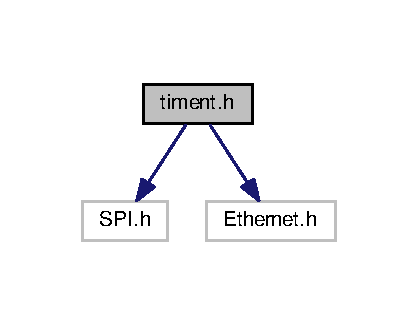
\includegraphics[width=201pt]{timent_8h__incl}
\end{center}
\end{figure}
This graph shows which files directly or indirectly include this file\+:
\nopagebreak
\begin{figure}[H]
\begin{center}
\leavevmode
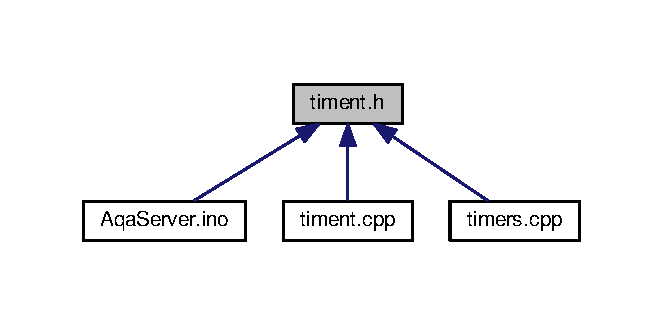
\includegraphics[width=318pt]{timent_8h__dep__incl}
\end{center}
\end{figure}
\subsection*{Functions}
\begin{DoxyCompactItemize}
\item 
void \hyperlink{timent_8h_ac1b08325eae558a954161be4af0f81e1}{init\+Timent} ()
\begin{DoxyCompactList}\small\item\em Init of R\+T\+C. \end{DoxyCompactList}\item 
byte \hyperlink{timent_8h_a825d19190ddbe72ed1536d48a6a23229}{dec\+To\+Bcd} (byte val)
\begin{DoxyCompactList}\small\item\em Decadic format to binary coded decimal. \end{DoxyCompactList}\item 
byte \hyperlink{timent_8h_a212db7b7699776a934657711a6a77d9b}{bcd\+To\+Dec} (byte val)
\begin{DoxyCompactList}\small\item\em Binary coded decimal to decadic format. \end{DoxyCompactList}\item 
void \hyperlink{timent_8h_a04e328e25f7ec25f880cfa590b0d2cc0}{set\+D\+S3231time} (byte second, byte \hyperlink{timers_8cpp_a0f100646613882af0415f3d97bd67875}{minute}, byte \hyperlink{timers_8cpp_aafa4b28cd4cce6ab8fbe430b55b647ad}{hour}, byte day\+Of\+Week, byte day\+Of\+Month, byte month, byte year)
\begin{DoxyCompactList}\small\item\em Setter for R\+T\+C. \end{DoxyCompactList}\item 
void \hyperlink{timent_8h_a2dc0bfb9c1fa2b144186ae2933d589ea}{read\+D\+S3231\+Minutes\+Houres} (byte $\ast$\hyperlink{timers_8cpp_a0f100646613882af0415f3d97bd67875}{minute}, byte $\ast$\hyperlink{timers_8cpp_aafa4b28cd4cce6ab8fbe430b55b647ad}{hour})
\item 
void \hyperlink{timent_8h_a2fb4d2d1f9d3145dcbe0c66f7152b48b}{read\+D\+S3231time} (byte $\ast$second, byte $\ast$\hyperlink{timers_8cpp_a0f100646613882af0415f3d97bd67875}{minute}, byte $\ast$\hyperlink{timers_8cpp_aafa4b28cd4cce6ab8fbe430b55b647ad}{hour}, byte $\ast$day\+Of\+Week, byte $\ast$day\+Of\+Month, byte $\ast$month, byte $\ast$year)
\item 
void \hyperlink{timent_8h_ad33063e0b5afbf35c57332e16881c0e7}{display\+Http\+Time} (Ethernet\+Client $\ast$client)
\begin{DoxyCompactList}\small\item\em Response for ethernet connection for time values. \end{DoxyCompactList}\item 
void \hyperlink{timent_8h_ab2f29739b10ddbedf9da6febe9c75917}{display\+Time} ()
\begin{DoxyCompactList}\small\item\em Displays time on the console. \end{DoxyCompactList}\item 
unsigned long \hyperlink{timent_8h_a12e5fa8d1663729d683386268d6fb233}{send\+N\+T\+Ppacket} (byte $\ast$address)
\begin{DoxyCompactList}\small\item\em Sender of N\+T\+P request to N\+T\+P server given by address. \end{DoxyCompactList}\item 
boolean \hyperlink{timent_8h_af20803fe4cebd4e2fc6a8062c32e865f}{set\+Time} ()
\begin{DoxyCompactList}\small\item\em Set time by N\+T\+P server to R\+T\+C. \end{DoxyCompactList}\end{DoxyCompactItemize}


\subsection{Function Documentation}
\hypertarget{timent_8h_a212db7b7699776a934657711a6a77d9b}{\index{timent.\+h@{timent.\+h}!bcd\+To\+Dec@{bcd\+To\+Dec}}
\index{bcd\+To\+Dec@{bcd\+To\+Dec}!timent.\+h@{timent.\+h}}
\subsubsection[{bcd\+To\+Dec}]{\setlength{\rightskip}{0pt plus 5cm}byte bcd\+To\+Dec (
\begin{DoxyParamCaption}
\item[{byte}]{val}
\end{DoxyParamCaption}
)}}\label{timent_8h_a212db7b7699776a934657711a6a77d9b}


Binary coded decimal to decadic format. 


\begin{DoxyParams}{Parameters}
{\em val} & Binary coded number. \\
\hline
\end{DoxyParams}
\begin{DoxyReturn}{Returns}
Decimal value. 
\end{DoxyReturn}


Definition at line 32 of file timent.\+cpp.

\hypertarget{timent_8h_a825d19190ddbe72ed1536d48a6a23229}{\index{timent.\+h@{timent.\+h}!dec\+To\+Bcd@{dec\+To\+Bcd}}
\index{dec\+To\+Bcd@{dec\+To\+Bcd}!timent.\+h@{timent.\+h}}
\subsubsection[{dec\+To\+Bcd}]{\setlength{\rightskip}{0pt plus 5cm}byte dec\+To\+Bcd (
\begin{DoxyParamCaption}
\item[{byte}]{val}
\end{DoxyParamCaption}
)}}\label{timent_8h_a825d19190ddbe72ed1536d48a6a23229}


Decadic format to binary coded decimal. 


\begin{DoxyParams}{Parameters}
{\em val} & Decadic number \\
\hline
\end{DoxyParams}
\begin{DoxyReturn}{Returns}
Binary coded decimal value. 
\end{DoxyReturn}


Definition at line 27 of file timent.\+cpp.

\hypertarget{timent_8h_ad33063e0b5afbf35c57332e16881c0e7}{\index{timent.\+h@{timent.\+h}!display\+Http\+Time@{display\+Http\+Time}}
\index{display\+Http\+Time@{display\+Http\+Time}!timent.\+h@{timent.\+h}}
\subsubsection[{display\+Http\+Time}]{\setlength{\rightskip}{0pt plus 5cm}void display\+Http\+Time (
\begin{DoxyParamCaption}
\item[{Ethernet\+Client $\ast$}]{client}
\end{DoxyParamCaption}
)}}\label{timent_8h_ad33063e0b5afbf35c57332e16881c0e7}


Response for ethernet connection for time values. 


\begin{DoxyParams}{Parameters}
{\em client} & Ethernet client to send the message to. \\
\hline
\end{DoxyParams}


Definition at line 75 of file timent.\+cpp.

\hypertarget{timent_8h_ab2f29739b10ddbedf9da6febe9c75917}{\index{timent.\+h@{timent.\+h}!display\+Time@{display\+Time}}
\index{display\+Time@{display\+Time}!timent.\+h@{timent.\+h}}
\subsubsection[{display\+Time}]{\setlength{\rightskip}{0pt plus 5cm}void display\+Time (
\begin{DoxyParamCaption}
{}
\end{DoxyParamCaption}
)}}\label{timent_8h_ab2f29739b10ddbedf9da6febe9c75917}


Displays time on the console. 



Definition at line 124 of file timent.\+cpp.

\hypertarget{timent_8h_ac1b08325eae558a954161be4af0f81e1}{\index{timent.\+h@{timent.\+h}!init\+Timent@{init\+Timent}}
\index{init\+Timent@{init\+Timent}!timent.\+h@{timent.\+h}}
\subsubsection[{init\+Timent}]{\setlength{\rightskip}{0pt plus 5cm}void init\+Timent (
\begin{DoxyParamCaption}
{}
\end{DoxyParamCaption}
)}}\label{timent_8h_ac1b08325eae558a954161be4af0f81e1}


Init of R\+T\+C. 



Definition at line 23 of file timent.\+cpp.

\hypertarget{timent_8h_a2dc0bfb9c1fa2b144186ae2933d589ea}{\index{timent.\+h@{timent.\+h}!read\+D\+S3231\+Minutes\+Houres@{read\+D\+S3231\+Minutes\+Houres}}
\index{read\+D\+S3231\+Minutes\+Houres@{read\+D\+S3231\+Minutes\+Houres}!timent.\+h@{timent.\+h}}
\subsubsection[{read\+D\+S3231\+Minutes\+Houres}]{\setlength{\rightskip}{0pt plus 5cm}void read\+D\+S3231\+Minutes\+Houres (
\begin{DoxyParamCaption}
\item[{byte $\ast$}]{minute, }
\item[{byte $\ast$}]{hour}
\end{DoxyParamCaption}
)}}\label{timent_8h_a2dc0bfb9c1fa2b144186ae2933d589ea}


Definition at line 49 of file timent.\+cpp.

\hypertarget{timent_8h_a2fb4d2d1f9d3145dcbe0c66f7152b48b}{\index{timent.\+h@{timent.\+h}!read\+D\+S3231time@{read\+D\+S3231time}}
\index{read\+D\+S3231time@{read\+D\+S3231time}!timent.\+h@{timent.\+h}}
\subsubsection[{read\+D\+S3231time}]{\setlength{\rightskip}{0pt plus 5cm}void read\+D\+S3231time (
\begin{DoxyParamCaption}
\item[{byte $\ast$}]{second, }
\item[{byte $\ast$}]{minute, }
\item[{byte $\ast$}]{hour, }
\item[{byte $\ast$}]{day\+Of\+Week, }
\item[{byte $\ast$}]{day\+Of\+Month, }
\item[{byte $\ast$}]{month, }
\item[{byte $\ast$}]{year}
\end{DoxyParamCaption}
)}}\label{timent_8h_a2fb4d2d1f9d3145dcbe0c66f7152b48b}


Definition at line 60 of file timent.\+cpp.

\hypertarget{timent_8h_a12e5fa8d1663729d683386268d6fb233}{\index{timent.\+h@{timent.\+h}!send\+N\+T\+Ppacket@{send\+N\+T\+Ppacket}}
\index{send\+N\+T\+Ppacket@{send\+N\+T\+Ppacket}!timent.\+h@{timent.\+h}}
\subsubsection[{send\+N\+T\+Ppacket}]{\setlength{\rightskip}{0pt plus 5cm}unsigned long send\+N\+T\+Ppacket (
\begin{DoxyParamCaption}
\item[{byte $\ast$}]{address}
\end{DoxyParamCaption}
)}}\label{timent_8h_a12e5fa8d1663729d683386268d6fb233}


Sender of N\+T\+P request to N\+T\+P server given by address. 


\begin{DoxyParams}{Parameters}
{\em address} & Address of N\+T\+P server. \\
\hline
\end{DoxyParams}
\begin{DoxyReturn}{Returns}
N\+T\+P time stamp. 
\end{DoxyReturn}


Definition at line 174 of file timent.\+cpp.

\hypertarget{timent_8h_a04e328e25f7ec25f880cfa590b0d2cc0}{\index{timent.\+h@{timent.\+h}!set\+D\+S3231time@{set\+D\+S3231time}}
\index{set\+D\+S3231time@{set\+D\+S3231time}!timent.\+h@{timent.\+h}}
\subsubsection[{set\+D\+S3231time}]{\setlength{\rightskip}{0pt plus 5cm}void set\+D\+S3231time (
\begin{DoxyParamCaption}
\item[{byte}]{second, }
\item[{byte}]{minute, }
\item[{byte}]{hour, }
\item[{byte}]{day\+Of\+Week, }
\item[{byte}]{day\+Of\+Month, }
\item[{byte}]{month, }
\item[{byte}]{year}
\end{DoxyParamCaption}
)}}\label{timent_8h_a04e328e25f7ec25f880cfa590b0d2cc0}


Setter for R\+T\+C. 


\begin{DoxyParams}{Parameters}
{\em second} & Second of time. \\
\hline
{\em minute} & Minute of time. \\
\hline
{\em hour} & Hours of time \\
\hline
{\em day\+Of\+Week} & Day of the week. \\
\hline
{\em day\+Of\+Month} & Day of the month. \\
\hline
{\em month} & Current month. \\
\hline
{\em year} & Current year. \\
\hline
\end{DoxyParams}


Definition at line 35 of file timent.\+cpp.

\hypertarget{timent_8h_af20803fe4cebd4e2fc6a8062c32e865f}{\index{timent.\+h@{timent.\+h}!set\+Time@{set\+Time}}
\index{set\+Time@{set\+Time}!timent.\+h@{timent.\+h}}
\subsubsection[{set\+Time}]{\setlength{\rightskip}{0pt plus 5cm}boolean set\+Time (
\begin{DoxyParamCaption}
{}
\end{DoxyParamCaption}
)}}\label{timent_8h_af20803fe4cebd4e2fc6a8062c32e865f}


Set time by N\+T\+P server to R\+T\+C. 

\begin{DoxyReturn}{Returns}
Status of time setting. 
\end{DoxyReturn}


Definition at line 194 of file timent.\+cpp.


\hypertarget{timers_8cpp}{\section{timers.\+cpp File Reference}
\label{timers_8cpp}\index{timers.\+cpp@{timers.\+cpp}}
}
{\ttfamily \#include \char`\"{}timers.\+h\char`\"{}}\\*
{\ttfamily \#include $<$Arduino.\+h$>$}\\*
{\ttfamily \#include $<$E\+E\+P\+R\+O\+M.\+h$>$}\\*
{\ttfamily \#include \char`\"{}timent.\+h\char`\"{}}\\*
{\ttfamily \#include \char`\"{}feeder.\+h\char`\"{}}\\*
{\ttfamily \#include \char`\"{}temp.\+h\char`\"{}}\\*
{\ttfamily \#include \char`\"{}relay.\+h\char`\"{}}\\*
Include dependency graph for timers.\+cpp\+:
\nopagebreak
\begin{figure}[H]
\begin{center}
\leavevmode
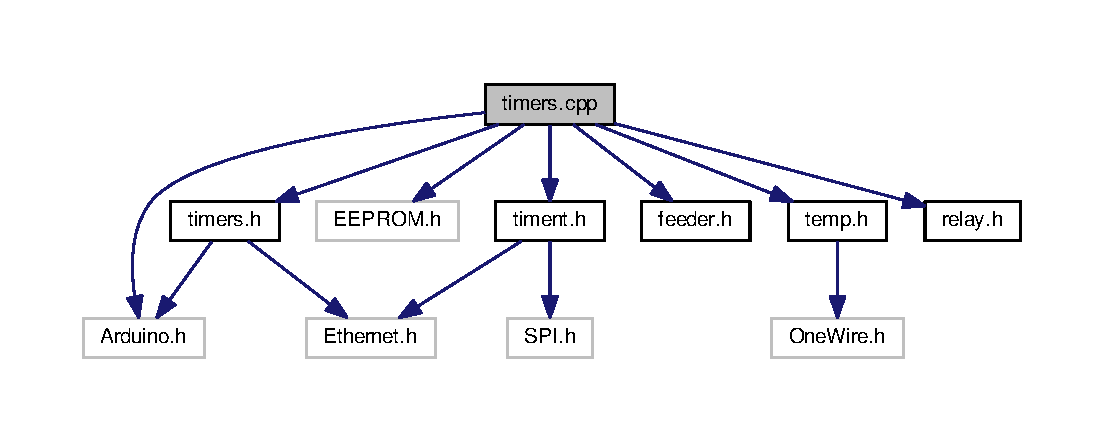
\includegraphics[width=350pt]{timers_8cpp__incl}
\end{center}
\end{figure}
\subsection*{Functions}
\begin{DoxyCompactItemize}
\item 
void \hyperlink{timers_8cpp_a9bfe70d722721ac4cd1e9dafc0ac5f17}{set\+Timers} ()
\begin{DoxyCompactList}\small\item\em Read R\+T\+C minute \& hour values. \end{DoxyCompactList}\item 
void \hyperlink{timers_8cpp_a8f1e7673ec5bbe382596c8c5b1c2c938}{check\+Temp\+Fr\+Min} (int heater)
\begin{DoxyCompactList}\small\item\em Check temperature in intervals. \end{DoxyCompactList}\item 
void \hyperlink{timers_8cpp_a096176edca3be6491fe26a8f967d0aee}{feed\+Fish} ()
\begin{DoxyCompactList}\small\item\em Feeds fish in aquarium. \end{DoxyCompactList}\item 
void \hyperlink{timers_8cpp_afd5128221c620ce341dc1254cf33b65d}{read\+Konst\+Val} ()
\begin{DoxyCompactList}\small\item\em Read E\+E\+P\+R\+O\+M values and set time time values for aqarium. \end{DoxyCompactList}\item 
bool \hyperlink{timers_8cpp_a962973b24f69e6a65d8b1597de2a1fb3}{set\+Tempr} (char $\ast$input)
\begin{DoxyCompactList}\small\item\em Set wish temperature of aquarium. \end{DoxyCompactList}\item 
void \hyperlink{timers_8cpp_a50ebb5a7c99715d386c2515a7abd21e4}{check\+Temp} (int heater)
\begin{DoxyCompactList}\small\item\em Check temperature. \end{DoxyCompactList}\item 
boolean \hyperlink{timers_8cpp_abbca993699ee6790390c692cdabf6fc2}{set\+E\+E\+Time} (char $\ast$input)
\begin{DoxyCompactList}\small\item\em Setup of time in E\+E\+P\+R\+O\+M. \end{DoxyCompactList}\item 
unsigned int \hyperlink{timers_8cpp_af49a30de967c5809446d449953a964e7}{get\+Wish\+Temp} ()
\begin{DoxyCompactList}\small\item\em Getter for wish temperature in tank. \end{DoxyCompactList}\item 
void \hyperlink{timers_8cpp_a48bf981461a55d8b282446ab81097da7}{setup\+Times} (int lights, int filter)
\begin{DoxyCompactList}\small\item\em Seting up pins by current time. \end{DoxyCompactList}\item 
void \hyperlink{timers_8cpp_a47ef6f0ac340d5be5d1c5d6ac4ee9885}{display\+Http\+Wake\+Time} (Ethernet\+Client $\ast$client)
\begin{DoxyCompactList}\small\item\em Response for ethernet connection for wake time values. \end{DoxyCompactList}\item 
void \hyperlink{timers_8cpp_a58ca77cf346143757c1f620e4cf280bc}{display\+Http\+Sleep\+Time} (Ethernet\+Client $\ast$client)
\begin{DoxyCompactList}\small\item\em Response for ethernet connection for sleep time values. \end{DoxyCompactList}\item 
void \hyperlink{timers_8cpp_a41c8b0d051898bad34f5d56d8df46215}{display\+Http\+Feed\+Time} (Ethernet\+Client $\ast$client)
\begin{DoxyCompactList}\small\item\em Response for ethernet connection for feep time values. \end{DoxyCompactList}\end{DoxyCompactItemize}
\subsection*{Variables}
\begin{DoxyCompactItemize}
\item 
\hyperlink{struct_tmr}{Tmr} \hyperlink{timers_8cpp_a061651429990c6c3a0443a7e56b21d89}{wake}
\begin{DoxyCompactList}\small\item\em Aquarium wake time. \end{DoxyCompactList}\item 
\hyperlink{struct_tmr}{Tmr} \hyperlink{timers_8cpp_a32db4ce90d7eb46b35f914dbde71cf5a}{endt}
\begin{DoxyCompactList}\small\item\em Aquarium sleep time. \end{DoxyCompactList}\item 
\hyperlink{struct_tmr}{Tmr} \hyperlink{timers_8cpp_a700359103e1dc784699671479b9153d2}{feedt}
\begin{DoxyCompactList}\small\item\em Aquarium feed time. \end{DoxyCompactList}\item 
int \hyperlink{timers_8cpp_a731d99156a30db9569dd34f137a4ff34}{tank\+Tmpr}
\begin{DoxyCompactList}\small\item\em Aquarium wish temperature. \end{DoxyCompactList}\item 
byte \hyperlink{timers_8cpp_a0f100646613882af0415f3d97bd67875}{minute}
\begin{DoxyCompactList}\small\item\em Current aquarium minute time. \end{DoxyCompactList}\item 
byte \hyperlink{timers_8cpp_aafa4b28cd4cce6ab8fbe430b55b647ad}{hour}
\begin{DoxyCompactList}\small\item\em Current aquarium minute time. \end{DoxyCompactList}\item 
boolean \hyperlink{timers_8cpp_a3e95f44a744553aaaca80a81b06c4bf2}{checktemp} = true
\end{DoxyCompactItemize}


\subsection{Function Documentation}
\hypertarget{timers_8cpp_a50ebb5a7c99715d386c2515a7abd21e4}{\index{timers.\+cpp@{timers.\+cpp}!check\+Temp@{check\+Temp}}
\index{check\+Temp@{check\+Temp}!timers.\+cpp@{timers.\+cpp}}
\subsubsection[{check\+Temp}]{\setlength{\rightskip}{0pt plus 5cm}check\+Temp (
\begin{DoxyParamCaption}
\item[{int}]{heater}
\end{DoxyParamCaption}
)}}\label{timers_8cpp_a50ebb5a7c99715d386c2515a7abd21e4}


Check temperature. 


\begin{DoxyParams}{Parameters}
{\em heater} & Heater pin number. \\
\hline
\end{DoxyParams}


Definition at line 79 of file timers.\+cpp.

\hypertarget{timers_8cpp_a8f1e7673ec5bbe382596c8c5b1c2c938}{\index{timers.\+cpp@{timers.\+cpp}!check\+Temp\+Fr\+Min@{check\+Temp\+Fr\+Min}}
\index{check\+Temp\+Fr\+Min@{check\+Temp\+Fr\+Min}!timers.\+cpp@{timers.\+cpp}}
\subsubsection[{check\+Temp\+Fr\+Min}]{\setlength{\rightskip}{0pt plus 5cm}check\+Temp\+Fr\+Min (
\begin{DoxyParamCaption}
\item[{int}]{heater}
\end{DoxyParamCaption}
)}}\label{timers_8cpp_a8f1e7673ec5bbe382596c8c5b1c2c938}


Check temperature in intervals. 


\begin{DoxyParams}{Parameters}
{\em heater} & Heater pin number. \\
\hline
\end{DoxyParams}


Definition at line 26 of file timers.\+cpp.

\hypertarget{timers_8cpp_a41c8b0d051898bad34f5d56d8df46215}{\index{timers.\+cpp@{timers.\+cpp}!display\+Http\+Feed\+Time@{display\+Http\+Feed\+Time}}
\index{display\+Http\+Feed\+Time@{display\+Http\+Feed\+Time}!timers.\+cpp@{timers.\+cpp}}
\subsubsection[{display\+Http\+Feed\+Time}]{\setlength{\rightskip}{0pt plus 5cm}display\+Http\+Feed\+Time (
\begin{DoxyParamCaption}
\item[{Ethernet\+Client $\ast$}]{client}
\end{DoxyParamCaption}
)}}\label{timers_8cpp_a41c8b0d051898bad34f5d56d8df46215}


Response for ethernet connection for feep time values. 


\begin{DoxyParams}{Parameters}
{\em client} & Ethernet client to send the message to. \\
\hline
\end{DoxyParams}


Definition at line 151 of file timers.\+cpp.

\hypertarget{timers_8cpp_a58ca77cf346143757c1f620e4cf280bc}{\index{timers.\+cpp@{timers.\+cpp}!display\+Http\+Sleep\+Time@{display\+Http\+Sleep\+Time}}
\index{display\+Http\+Sleep\+Time@{display\+Http\+Sleep\+Time}!timers.\+cpp@{timers.\+cpp}}
\subsubsection[{display\+Http\+Sleep\+Time}]{\setlength{\rightskip}{0pt plus 5cm}display\+Http\+Sleep\+Time (
\begin{DoxyParamCaption}
\item[{Ethernet\+Client $\ast$}]{client}
\end{DoxyParamCaption}
)}}\label{timers_8cpp_a58ca77cf346143757c1f620e4cf280bc}


Response for ethernet connection for sleep time values. 


\begin{DoxyParams}{Parameters}
{\em client} & Ethernet client to send the message to. \\
\hline
\end{DoxyParams}


Definition at line 144 of file timers.\+cpp.

\hypertarget{timers_8cpp_a47ef6f0ac340d5be5d1c5d6ac4ee9885}{\index{timers.\+cpp@{timers.\+cpp}!display\+Http\+Wake\+Time@{display\+Http\+Wake\+Time}}
\index{display\+Http\+Wake\+Time@{display\+Http\+Wake\+Time}!timers.\+cpp@{timers.\+cpp}}
\subsubsection[{display\+Http\+Wake\+Time}]{\setlength{\rightskip}{0pt plus 5cm}display\+Http\+Wake\+Time (
\begin{DoxyParamCaption}
\item[{Ethernet\+Client $\ast$}]{client}
\end{DoxyParamCaption}
)}}\label{timers_8cpp_a47ef6f0ac340d5be5d1c5d6ac4ee9885}


Response for ethernet connection for wake time values. 


\begin{DoxyParams}{Parameters}
{\em client} & Ethernet client to send the message to. \\
\hline
\end{DoxyParams}


Definition at line 137 of file timers.\+cpp.

\hypertarget{timers_8cpp_a096176edca3be6491fe26a8f967d0aee}{\index{timers.\+cpp@{timers.\+cpp}!feed\+Fish@{feed\+Fish}}
\index{feed\+Fish@{feed\+Fish}!timers.\+cpp@{timers.\+cpp}}
\subsubsection[{feed\+Fish}]{\setlength{\rightskip}{0pt plus 5cm}feed\+Fish (
\begin{DoxyParamCaption}
{}
\end{DoxyParamCaption}
)}}\label{timers_8cpp_a096176edca3be6491fe26a8f967d0aee}


Feeds fish in aquarium. 



Definition at line 35 of file timers.\+cpp.

\hypertarget{timers_8cpp_af49a30de967c5809446d449953a964e7}{\index{timers.\+cpp@{timers.\+cpp}!get\+Wish\+Temp@{get\+Wish\+Temp}}
\index{get\+Wish\+Temp@{get\+Wish\+Temp}!timers.\+cpp@{timers.\+cpp}}
\subsubsection[{get\+Wish\+Temp}]{\setlength{\rightskip}{0pt plus 5cm}get\+Wish\+Temp (
\begin{DoxyParamCaption}
{}
\end{DoxyParamCaption}
)}}\label{timers_8cpp_af49a30de967c5809446d449953a964e7}


Getter for wish temperature in tank. 

\begin{DoxyReturn}{Returns}
Wish temperature. 
\end{DoxyReturn}


Definition at line 119 of file timers.\+cpp.

\hypertarget{timers_8cpp_afd5128221c620ce341dc1254cf33b65d}{\index{timers.\+cpp@{timers.\+cpp}!read\+Konst\+Val@{read\+Konst\+Val}}
\index{read\+Konst\+Val@{read\+Konst\+Val}!timers.\+cpp@{timers.\+cpp}}
\subsubsection[{read\+Konst\+Val}]{\setlength{\rightskip}{0pt plus 5cm}read\+Konst\+Val (
\begin{DoxyParamCaption}
{}
\end{DoxyParamCaption}
)}}\label{timers_8cpp_afd5128221c620ce341dc1254cf33b65d}


Read E\+E\+P\+R\+O\+M values and set time time values for aqarium. 



Definition at line 44 of file timers.\+cpp.

\hypertarget{timers_8cpp_abbca993699ee6790390c692cdabf6fc2}{\index{timers.\+cpp@{timers.\+cpp}!set\+E\+E\+Time@{set\+E\+E\+Time}}
\index{set\+E\+E\+Time@{set\+E\+E\+Time}!timers.\+cpp@{timers.\+cpp}}
\subsubsection[{set\+E\+E\+Time}]{\setlength{\rightskip}{0pt plus 5cm}set\+E\+E\+Time (
\begin{DoxyParamCaption}
\item[{char $\ast$}]{input}
\end{DoxyParamCaption}
)}}\label{timers_8cpp_abbca993699ee6790390c692cdabf6fc2}


Setup of time in E\+E\+P\+R\+O\+M. 


\begin{DoxyParams}{Parameters}
{\em input} & Time to store in E\+E\+P\+R\+O\+M. \\
\hline
\end{DoxyParams}
\begin{DoxyReturn}{Returns}
Statues of stored values. 
\end{DoxyReturn}


Definition at line 87 of file timers.\+cpp.

\hypertarget{timers_8cpp_a962973b24f69e6a65d8b1597de2a1fb3}{\index{timers.\+cpp@{timers.\+cpp}!set\+Tempr@{set\+Tempr}}
\index{set\+Tempr@{set\+Tempr}!timers.\+cpp@{timers.\+cpp}}
\subsubsection[{set\+Tempr}]{\setlength{\rightskip}{0pt plus 5cm}set\+Tempr (
\begin{DoxyParamCaption}
\item[{char $\ast$}]{input}
\end{DoxyParamCaption}
)}}\label{timers_8cpp_a962973b24f69e6a65d8b1597de2a1fb3}


Set wish temperature of aquarium. 


\begin{DoxyParams}{Parameters}
{\em input} & Input of readed chars \\
\hline
\end{DoxyParams}
\begin{DoxyReturn}{Returns}
Statues of written data. 
\end{DoxyReturn}


Definition at line 72 of file timers.\+cpp.

\hypertarget{timers_8cpp_a9bfe70d722721ac4cd1e9dafc0ac5f17}{\index{timers.\+cpp@{timers.\+cpp}!set\+Timers@{set\+Timers}}
\index{set\+Timers@{set\+Timers}!timers.\+cpp@{timers.\+cpp}}
\subsubsection[{set\+Timers}]{\setlength{\rightskip}{0pt plus 5cm}set\+Timers (
\begin{DoxyParamCaption}
{}
\end{DoxyParamCaption}
)}}\label{timers_8cpp_a9bfe70d722721ac4cd1e9dafc0ac5f17}


Read R\+T\+C minute \& hour values. 



Definition at line 22 of file timers.\+cpp.

\hypertarget{timers_8cpp_a48bf981461a55d8b282446ab81097da7}{\index{timers.\+cpp@{timers.\+cpp}!setup\+Times@{setup\+Times}}
\index{setup\+Times@{setup\+Times}!timers.\+cpp@{timers.\+cpp}}
\subsubsection[{setup\+Times}]{\setlength{\rightskip}{0pt plus 5cm}setup\+Times (
\begin{DoxyParamCaption}
\item[{int}]{lights, }
\item[{int}]{filter}
\end{DoxyParamCaption}
)}}\label{timers_8cpp_a48bf981461a55d8b282446ab81097da7}


Seting up pins by current time. 


\begin{DoxyParams}{Parameters}
{\em lights} & Lights pin value. \\
\hline
{\em filter} & Filter pin value. \\
\hline
\end{DoxyParams}


Definition at line 123 of file timers.\+cpp.



\subsection{Variable Documentation}
\hypertarget{timers_8cpp_a3e95f44a744553aaaca80a81b06c4bf2}{\index{timers.\+cpp@{timers.\+cpp}!checktemp@{checktemp}}
\index{checktemp@{checktemp}!timers.\+cpp@{timers.\+cpp}}
\subsubsection[{checktemp}]{\setlength{\rightskip}{0pt plus 5cm}boolean checktemp = true}}\label{timers_8cpp_a3e95f44a744553aaaca80a81b06c4bf2}


Definition at line 17 of file timers.\+cpp.

\hypertarget{timers_8cpp_a32db4ce90d7eb46b35f914dbde71cf5a}{\index{timers.\+cpp@{timers.\+cpp}!endt@{endt}}
\index{endt@{endt}!timers.\+cpp@{timers.\+cpp}}
\subsubsection[{endt}]{\setlength{\rightskip}{0pt plus 5cm}{\bf Tmr} endt}}\label{timers_8cpp_a32db4ce90d7eb46b35f914dbde71cf5a}


Aquarium sleep time. 



Definition at line 10 of file timers.\+cpp.

\hypertarget{timers_8cpp_a700359103e1dc784699671479b9153d2}{\index{timers.\+cpp@{timers.\+cpp}!feedt@{feedt}}
\index{feedt@{feedt}!timers.\+cpp@{timers.\+cpp}}
\subsubsection[{feedt}]{\setlength{\rightskip}{0pt plus 5cm}{\bf Tmr} feedt}}\label{timers_8cpp_a700359103e1dc784699671479b9153d2}


Aquarium feed time. 



Definition at line 11 of file timers.\+cpp.

\hypertarget{timers_8cpp_aafa4b28cd4cce6ab8fbe430b55b647ad}{\index{timers.\+cpp@{timers.\+cpp}!hour@{hour}}
\index{hour@{hour}!timers.\+cpp@{timers.\+cpp}}
\subsubsection[{hour}]{\setlength{\rightskip}{0pt plus 5cm}byte hour}}\label{timers_8cpp_aafa4b28cd4cce6ab8fbe430b55b647ad}


Current aquarium minute time. 



Definition at line 15 of file timers.\+cpp.

\hypertarget{timers_8cpp_a0f100646613882af0415f3d97bd67875}{\index{timers.\+cpp@{timers.\+cpp}!minute@{minute}}
\index{minute@{minute}!timers.\+cpp@{timers.\+cpp}}
\subsubsection[{minute}]{\setlength{\rightskip}{0pt plus 5cm}byte minute}}\label{timers_8cpp_a0f100646613882af0415f3d97bd67875}


Current aquarium minute time. 



Definition at line 14 of file timers.\+cpp.

\hypertarget{timers_8cpp_a731d99156a30db9569dd34f137a4ff34}{\index{timers.\+cpp@{timers.\+cpp}!tank\+Tmpr@{tank\+Tmpr}}
\index{tank\+Tmpr@{tank\+Tmpr}!timers.\+cpp@{timers.\+cpp}}
\subsubsection[{tank\+Tmpr}]{\setlength{\rightskip}{0pt plus 5cm}int tank\+Tmpr}}\label{timers_8cpp_a731d99156a30db9569dd34f137a4ff34}


Aquarium wish temperature. 



Definition at line 12 of file timers.\+cpp.

\hypertarget{timers_8cpp_a061651429990c6c3a0443a7e56b21d89}{\index{timers.\+cpp@{timers.\+cpp}!wake@{wake}}
\index{wake@{wake}!timers.\+cpp@{timers.\+cpp}}
\subsubsection[{wake}]{\setlength{\rightskip}{0pt plus 5cm}{\bf Tmr} wake}}\label{timers_8cpp_a061651429990c6c3a0443a7e56b21d89}


Aquarium wake time. 



Definition at line 9 of file timers.\+cpp.


\hypertarget{timers_8h}{\section{timers.\+h File Reference}
\label{timers_8h}\index{timers.\+h@{timers.\+h}}
}
{\ttfamily \#include $<$Arduino.\+h$>$}\\*
{\ttfamily \#include $<$Ethernet.\+h$>$}\\*
Include dependency graph for timers.\+h\+:
\nopagebreak
\begin{figure}[H]
\begin{center}
\leavevmode
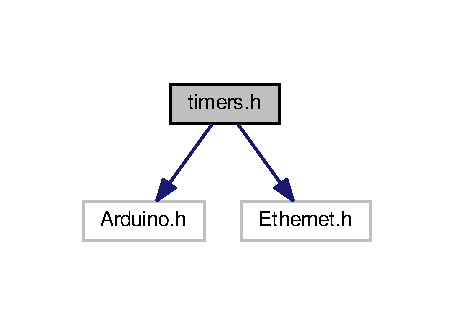
\includegraphics[width=218pt]{timers_8h__incl}
\end{center}
\end{figure}
This graph shows which files directly or indirectly include this file\+:
\nopagebreak
\begin{figure}[H]
\begin{center}
\leavevmode
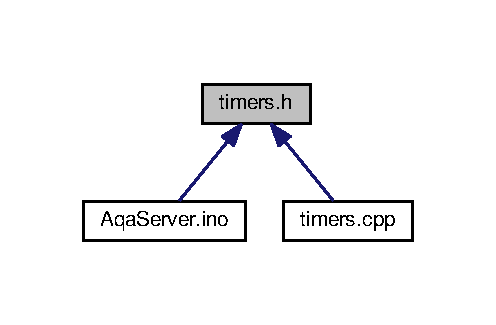
\includegraphics[width=238pt]{timers_8h__dep__incl}
\end{center}
\end{figure}
\subsection*{Classes}
\begin{DoxyCompactItemize}
\item 
class \hyperlink{struct_tmr}{Tmr}
\begin{DoxyCompactList}\small\item\em Timer class for containg timers like wake time or sleep time. \end{DoxyCompactList}\end{DoxyCompactItemize}
\subsection*{Functions}
\begin{DoxyCompactItemize}
\item 
void \hyperlink{timers_8h_a8c2d5f94de582dc8a661bc7ab7320921}{set\+Timers} ()
\begin{DoxyCompactList}\small\item\em Read R\+T\+C minute \& hour values. \end{DoxyCompactList}\item 
void \hyperlink{timers_8h_a6c462a1b8bb06e2c8b26e9b9184f6e5f}{read\+Konst\+Val} ()
\begin{DoxyCompactList}\small\item\em Read E\+E\+P\+R\+O\+M values and set time time values for aqarium. \end{DoxyCompactList}\item 
bool \hyperlink{timers_8h_af23df4b27d6bf43e18bd02906628971b}{set\+Tempr} (char $\ast$input)
\begin{DoxyCompactList}\small\item\em Set wish temperature of aquarium. \end{DoxyCompactList}\item 
void \hyperlink{timers_8h_ad1cb5d7c1c0d0e6d64d937f22f734490}{feed\+Fish} ()
\begin{DoxyCompactList}\small\item\em Feeds fish in aquarium. \end{DoxyCompactList}\item 
void \hyperlink{timers_8h_aa26c250f7c820c612fbee9db2bb7980a}{setup\+Times} (int lights, int filter)
\begin{DoxyCompactList}\small\item\em Seting up pins by current time. \end{DoxyCompactList}\item 
unsigned int \hyperlink{timers_8h_a1a36195e612019d37b51dc40de6bc782}{get\+Wish\+Temp} ()
\begin{DoxyCompactList}\small\item\em Getter for wish temperature in tank. \end{DoxyCompactList}\item 
void \hyperlink{timers_8h_aef55a87adaa35f6ecb887dce1706880b}{check\+Temp\+Fr\+Min} (int heater)
\begin{DoxyCompactList}\small\item\em Check temperature in intervals. \end{DoxyCompactList}\item 
void \hyperlink{timers_8h_a73d4e08cbcbf2836c53bcc9b1fc4b996}{check\+Temp} (int heater)
\begin{DoxyCompactList}\small\item\em Check temperature. \end{DoxyCompactList}\item 
boolean \hyperlink{timers_8h_accb5e0e138acbd16797cfa37e6929bc5}{set\+E\+E\+Time} (char $\ast$input)
\begin{DoxyCompactList}\small\item\em Setup of time in E\+E\+P\+R\+O\+M. \end{DoxyCompactList}\item 
void \hyperlink{timers_8h_a30fdedfd3701079c052a36896fa96afe}{display\+Http\+Wake\+Time} (Ethernet\+Client $\ast$client)
\begin{DoxyCompactList}\small\item\em Response for ethernet connection for wake time values. \end{DoxyCompactList}\item 
void \hyperlink{timers_8h_a385947ec0556b99e7feb441efe7461e7}{display\+Http\+Feed\+Time} (Ethernet\+Client $\ast$client)
\begin{DoxyCompactList}\small\item\em Response for ethernet connection for feep time values. \end{DoxyCompactList}\item 
void \hyperlink{timers_8h_ada6638e7a11d9e94edac324a7aed9ba7}{display\+Http\+Sleep\+Time} (Ethernet\+Client $\ast$client)
\begin{DoxyCompactList}\small\item\em Response for ethernet connection for sleep time values. \end{DoxyCompactList}\end{DoxyCompactItemize}


\subsection{Function Documentation}
\hypertarget{timers_8h_a73d4e08cbcbf2836c53bcc9b1fc4b996}{\index{timers.\+h@{timers.\+h}!check\+Temp@{check\+Temp}}
\index{check\+Temp@{check\+Temp}!timers.\+h@{timers.\+h}}
\subsubsection[{check\+Temp}]{\setlength{\rightskip}{0pt plus 5cm}void check\+Temp (
\begin{DoxyParamCaption}
\item[{int}]{heater}
\end{DoxyParamCaption}
)}}\label{timers_8h_a73d4e08cbcbf2836c53bcc9b1fc4b996}


Check temperature. 


\begin{DoxyParams}{Parameters}
{\em heater} & Heater pin number. \\
\hline
\end{DoxyParams}


Definition at line 79 of file timers.\+cpp.

\hypertarget{timers_8h_aef55a87adaa35f6ecb887dce1706880b}{\index{timers.\+h@{timers.\+h}!check\+Temp\+Fr\+Min@{check\+Temp\+Fr\+Min}}
\index{check\+Temp\+Fr\+Min@{check\+Temp\+Fr\+Min}!timers.\+h@{timers.\+h}}
\subsubsection[{check\+Temp\+Fr\+Min}]{\setlength{\rightskip}{0pt plus 5cm}void check\+Temp\+Fr\+Min (
\begin{DoxyParamCaption}
\item[{int}]{heater}
\end{DoxyParamCaption}
)}}\label{timers_8h_aef55a87adaa35f6ecb887dce1706880b}


Check temperature in intervals. 


\begin{DoxyParams}{Parameters}
{\em heater} & Heater pin number. \\
\hline
\end{DoxyParams}


Definition at line 26 of file timers.\+cpp.

\hypertarget{timers_8h_a385947ec0556b99e7feb441efe7461e7}{\index{timers.\+h@{timers.\+h}!display\+Http\+Feed\+Time@{display\+Http\+Feed\+Time}}
\index{display\+Http\+Feed\+Time@{display\+Http\+Feed\+Time}!timers.\+h@{timers.\+h}}
\subsubsection[{display\+Http\+Feed\+Time}]{\setlength{\rightskip}{0pt plus 5cm}void display\+Http\+Feed\+Time (
\begin{DoxyParamCaption}
\item[{Ethernet\+Client $\ast$}]{client}
\end{DoxyParamCaption}
)}}\label{timers_8h_a385947ec0556b99e7feb441efe7461e7}


Response for ethernet connection for feep time values. 


\begin{DoxyParams}{Parameters}
{\em client} & Ethernet client to send the message to. \\
\hline
\end{DoxyParams}


Definition at line 151 of file timers.\+cpp.

\hypertarget{timers_8h_ada6638e7a11d9e94edac324a7aed9ba7}{\index{timers.\+h@{timers.\+h}!display\+Http\+Sleep\+Time@{display\+Http\+Sleep\+Time}}
\index{display\+Http\+Sleep\+Time@{display\+Http\+Sleep\+Time}!timers.\+h@{timers.\+h}}
\subsubsection[{display\+Http\+Sleep\+Time}]{\setlength{\rightskip}{0pt plus 5cm}void display\+Http\+Sleep\+Time (
\begin{DoxyParamCaption}
\item[{Ethernet\+Client $\ast$}]{client}
\end{DoxyParamCaption}
)}}\label{timers_8h_ada6638e7a11d9e94edac324a7aed9ba7}


Response for ethernet connection for sleep time values. 


\begin{DoxyParams}{Parameters}
{\em client} & Ethernet client to send the message to. \\
\hline
\end{DoxyParams}


Definition at line 144 of file timers.\+cpp.

\hypertarget{timers_8h_a30fdedfd3701079c052a36896fa96afe}{\index{timers.\+h@{timers.\+h}!display\+Http\+Wake\+Time@{display\+Http\+Wake\+Time}}
\index{display\+Http\+Wake\+Time@{display\+Http\+Wake\+Time}!timers.\+h@{timers.\+h}}
\subsubsection[{display\+Http\+Wake\+Time}]{\setlength{\rightskip}{0pt plus 5cm}void display\+Http\+Wake\+Time (
\begin{DoxyParamCaption}
\item[{Ethernet\+Client $\ast$}]{client}
\end{DoxyParamCaption}
)}}\label{timers_8h_a30fdedfd3701079c052a36896fa96afe}


Response for ethernet connection for wake time values. 


\begin{DoxyParams}{Parameters}
{\em client} & Ethernet client to send the message to. \\
\hline
\end{DoxyParams}


Definition at line 137 of file timers.\+cpp.

\hypertarget{timers_8h_ad1cb5d7c1c0d0e6d64d937f22f734490}{\index{timers.\+h@{timers.\+h}!feed\+Fish@{feed\+Fish}}
\index{feed\+Fish@{feed\+Fish}!timers.\+h@{timers.\+h}}
\subsubsection[{feed\+Fish}]{\setlength{\rightskip}{0pt plus 5cm}void feed\+Fish (
\begin{DoxyParamCaption}
{}
\end{DoxyParamCaption}
)}}\label{timers_8h_ad1cb5d7c1c0d0e6d64d937f22f734490}


Feeds fish in aquarium. 



Definition at line 35 of file timers.\+cpp.

\hypertarget{timers_8h_a1a36195e612019d37b51dc40de6bc782}{\index{timers.\+h@{timers.\+h}!get\+Wish\+Temp@{get\+Wish\+Temp}}
\index{get\+Wish\+Temp@{get\+Wish\+Temp}!timers.\+h@{timers.\+h}}
\subsubsection[{get\+Wish\+Temp}]{\setlength{\rightskip}{0pt plus 5cm}unsigned int get\+Wish\+Temp (
\begin{DoxyParamCaption}
{}
\end{DoxyParamCaption}
)}}\label{timers_8h_a1a36195e612019d37b51dc40de6bc782}


Getter for wish temperature in tank. 

\begin{DoxyReturn}{Returns}
Wish temperature. 
\end{DoxyReturn}


Definition at line 119 of file timers.\+cpp.

\hypertarget{timers_8h_a6c462a1b8bb06e2c8b26e9b9184f6e5f}{\index{timers.\+h@{timers.\+h}!read\+Konst\+Val@{read\+Konst\+Val}}
\index{read\+Konst\+Val@{read\+Konst\+Val}!timers.\+h@{timers.\+h}}
\subsubsection[{read\+Konst\+Val}]{\setlength{\rightskip}{0pt plus 5cm}void read\+Konst\+Val (
\begin{DoxyParamCaption}
{}
\end{DoxyParamCaption}
)}}\label{timers_8h_a6c462a1b8bb06e2c8b26e9b9184f6e5f}


Read E\+E\+P\+R\+O\+M values and set time time values for aqarium. 



Definition at line 44 of file timers.\+cpp.

\hypertarget{timers_8h_accb5e0e138acbd16797cfa37e6929bc5}{\index{timers.\+h@{timers.\+h}!set\+E\+E\+Time@{set\+E\+E\+Time}}
\index{set\+E\+E\+Time@{set\+E\+E\+Time}!timers.\+h@{timers.\+h}}
\subsubsection[{set\+E\+E\+Time}]{\setlength{\rightskip}{0pt plus 5cm}boolean set\+E\+E\+Time (
\begin{DoxyParamCaption}
\item[{char $\ast$}]{input}
\end{DoxyParamCaption}
)}}\label{timers_8h_accb5e0e138acbd16797cfa37e6929bc5}


Setup of time in E\+E\+P\+R\+O\+M. 


\begin{DoxyParams}{Parameters}
{\em input} & Time to store in E\+E\+P\+R\+O\+M. \\
\hline
\end{DoxyParams}
\begin{DoxyReturn}{Returns}
Statues of stored values. 
\end{DoxyReturn}


Definition at line 87 of file timers.\+cpp.

\hypertarget{timers_8h_af23df4b27d6bf43e18bd02906628971b}{\index{timers.\+h@{timers.\+h}!set\+Tempr@{set\+Tempr}}
\index{set\+Tempr@{set\+Tempr}!timers.\+h@{timers.\+h}}
\subsubsection[{set\+Tempr}]{\setlength{\rightskip}{0pt plus 5cm}bool set\+Tempr (
\begin{DoxyParamCaption}
\item[{char $\ast$}]{input}
\end{DoxyParamCaption}
)}}\label{timers_8h_af23df4b27d6bf43e18bd02906628971b}


Set wish temperature of aquarium. 


\begin{DoxyParams}{Parameters}
{\em input} & Input of readed chars \\
\hline
\end{DoxyParams}
\begin{DoxyReturn}{Returns}
Statues of written data. 
\end{DoxyReturn}


Definition at line 72 of file timers.\+cpp.

\hypertarget{timers_8h_a8c2d5f94de582dc8a661bc7ab7320921}{\index{timers.\+h@{timers.\+h}!set\+Timers@{set\+Timers}}
\index{set\+Timers@{set\+Timers}!timers.\+h@{timers.\+h}}
\subsubsection[{set\+Timers}]{\setlength{\rightskip}{0pt plus 5cm}void set\+Timers (
\begin{DoxyParamCaption}
{}
\end{DoxyParamCaption}
)}}\label{timers_8h_a8c2d5f94de582dc8a661bc7ab7320921}


Read R\+T\+C minute \& hour values. 



Definition at line 22 of file timers.\+cpp.

\hypertarget{timers_8h_aa26c250f7c820c612fbee9db2bb7980a}{\index{timers.\+h@{timers.\+h}!setup\+Times@{setup\+Times}}
\index{setup\+Times@{setup\+Times}!timers.\+h@{timers.\+h}}
\subsubsection[{setup\+Times}]{\setlength{\rightskip}{0pt plus 5cm}void setup\+Times (
\begin{DoxyParamCaption}
\item[{int}]{lights, }
\item[{int}]{filter}
\end{DoxyParamCaption}
)}}\label{timers_8h_aa26c250f7c820c612fbee9db2bb7980a}


Seting up pins by current time. 


\begin{DoxyParams}{Parameters}
{\em lights} & Lights pin value. \\
\hline
{\em filter} & Filter pin value. \\
\hline
\end{DoxyParams}


Definition at line 123 of file timers.\+cpp.


%--- End generated contents ---

% Index
\newpage
\phantomsection
\addcontentsline{toc}{chapter}{Index}
\printindex

\end{document}
